
\chapter{The logic of types. I. Disjunctive types\label{chap:Disjunctive-types}}

Disjunctive types describe values that belong to a disjoint set of
alternatives. 

To see how Scala implements disjunctive types, we need to begin by
looking at \textsf{``}case classes\textsf{''}.

\section{Scala\textsf{'}s \textquotedblleft case classes\textquotedblright}

\subsection{Tuple types with names}

It is often helpful to use names for the different parts of a tuple.
Suppose that some program represents the size and the color of socks
with the tuple type \lstinline!(Double, String)!. What if the same
tuple type \lstinline!(Double, String)! is used in another place
in the program to mean the amount paid and the payee? A programmer
could mix the two values by mistake, and it would be hard to find
out why the program incorrectly computes, say, the total amount paid:
\begin{lstlisting}
def totalAmountPaid(ps: Seq[(Double, String)]): Double = ps.map(_._1).sum
val x = (10.5, "white")       // Sock size and color.
val y = (25.0, "restaurant")  // The amount paid and the payee.

scala> totalAmountPaid(Seq(x, y)) // Nonsense.
res0: Double = 35.5
\end{lstlisting}

We would prevent this kind of mistake if we could use two \emph{different}
types, with names such as \lstinline!MySock! and \lstinline!Payment!,
for the two kinds of data. There are  three basic ways of defining
a new named type in Scala: using a type alias, using a class (or \textsf{``}trait\textsf{''}),
and using an \index{opaque type}opaque type. 

Opaque types (hiding a type under a new name) is a feature of Scala
3. It can be seen as a case class with a single field but without
the cost of memory allocation. Here, we will focus on type aliases
and case classes.

A \textbf{type alias}\index{type alias} is an alternative name for
an existing (already defined) type. We could use type aliases in our
example to add clarity to the code:
\begin{lstlisting}
type MySockTuple = (Double, String)
type PaymentTuple = (Double, String)

scala> val s: MySockTuple = (10.5, "white")
s: MySockTuple = (10.5,white)

scala> val p: PaymentTuple = (25.0, "restaurant")
p: PaymentTuple = (25.0,restaurant)
\end{lstlisting}
But type aliases do not prevent mix-up errors:
\begin{lstlisting}
scala> totalAmountPaid(Seq(s, p)) // Nonsense again.
res1: Double = 35.5
\end{lstlisting}

Scala\textsf{'}s \textbf{case classes}\index{case class} can be seen as \textsf{``}tuples
with names\textsf{''}. A case class is equivalent to a tuple type that has
a name designating the type and a separate name for each part of the
case class. This is how we might define case classes for the example
with socks and payments:
\begin{lstlisting}
case class MySock(size: Double, color: String)
case class Payment(amount: Double, name: String)

scala> val sock = MySock(10.5, "white")
sock: MySock = MySock(10.5,white)

scala> val paid = Payment(25.0, "restaurant")
paid: Payment = Payment(25.0,restaurant)                                  
\end{lstlisting}
This code defines new types named \lstinline!MySock! and \lstinline!Payment!.
Values of type \lstinline!MySock! are written as \lstinline!MySock(10.5, "white")!,
which is similar to writing the tuple \lstinline!(10.5, "white")!
except for adding the name \lstinline!MySock! in front of the tuple.

To access the parts of a case class, we use the part names:
\begin{lstlisting}
scala> sock.size
res2: Double = 10.5

scala> paid.amount
res3: Double = 25.0
\end{lstlisting}
The mix-up error is now a \index{type error}type error detected by
the compiler:
\begin{lstlisting}
def totalAmountPaid(ps: Seq[Payment]): Double = ps.map(_.amount).sum

scala> totalAmountPaid(Seq(paid, paid))
res4: Double = 50.0

scala> totalAmountPaid(Seq(sock, paid))
<console>:19: error: type mismatch;
 found   : MySock
 required: Payment
       totalAmountPaid(Seq(sock, paid))
                           ^
\end{lstlisting}
A function whose argument is of type \lstinline!MySock! cannot be
applied to an argument of type \lstinline!Payment!. Case classes
with different names are \emph{different types}, even if they contain
the same parts. 

It is important that type errors are detected at compile time. Compiled
programs can run only if all types match. This prevents a broad class
of run-time errors that occur due to wrong types. 

Just as tuples can have any number of parts, case classes can have
any number of parts, but the part names must be distinct, for example:
\begin{lstlisting}
case class Person(firstName: String, lastName: String, age: Int)

scala> val noether = Person("Emmy", "Noether", 137)
noether: Person = Person(Emmy,Noether,137)

scala> noether.firstName
res5: String = Emmy

scala> noether.age
res6: Int = 137
\end{lstlisting}
This data type carries the same information as a tuple \lstinline!(String, String, Int)!.
However, the declaration of a \lstinline!case class Person! gives
the programmer several features that make working with the tuple\textsf{'}s
data more convenient and less error-prone.

Some (or all) part names may be specified when creating a case class
value:
\begin{lstlisting}[extendedchars=true,mathescape=true]
scala> val poincar$\text{\'e}$ = Person(firstName = "Henri", lastName = "Poincar$\text{\color{mauve}\'e}$", 165)
poincar$\text{\'{e}}$: Person = Person(Henri,Poincar$\text{\'e}$,165)
\end{lstlisting}
It is a type error to use wrong types with a case class:
\begin{lstlisting}
scala> val p = Person(140, "Einstein", "Albert")
<console>:13: error: type mismatch;
 found   : Int(140)
 required: String
       val p = Person(140, "Einstein", "Albert")
                      ^
<console>:13: error: type mismatch;
 found   : String("Albert")
 required: Int
       val p = Person(140, "Einstein", "Albert")
                                       ^
\end{lstlisting}
This error is due to an incorrect order of parts when creating a case
class value. However, parts can be specified in any order when using
part names:
\begin{lstlisting}
scala> val p = Person(age = 137, lastName = "Noether", firstName = "Emmy")
p: Person = Person(Emmy,Noether,137)
\end{lstlisting}
A part of a case class can have the type of another case class, creating
a type similar to a nested tuple:
\begin{lstlisting}
case class BagOfSocks(sock: MySock, count: Int)
val bag = BagOfSocks(MySock(10.5, "white"), 6)

scala> bag.sock.size
res7: Double = 10.5
\end{lstlisting}


\subsection{Case classes with type parameters}

Type classes can be defined with \index{type parameter}type parameters.
As an example, consider an extension of \lstinline!MySock! where,
in addition to the size and color, an \textsf{``}extended sock\textsf{''} holds another
value. We could define several specialized case classes:
\begin{lstlisting}
case class MySockInt(size: Double, color: String, value: Int)
case class MySockBoolean(size: Double, color: String, value: Boolean)
\end{lstlisting}
but it is better to define a single parameterized case class:
\begin{lstlisting}
case class MySockX[A](size: Double, color: String, value: A)
\end{lstlisting}
This case class can accommodate every type \lstinline!A!. We may
now create values of \lstinline!MySockX! containing a \lstinline!value!
of any given type, say \lstinline!Int!:
\begin{lstlisting}
scala> val s = MySockX(10.5, "white", 123)
s: MySockX[Int] = MySockX(10.5,white,123) 
\end{lstlisting}
Because the value \lstinline!123! has type \lstinline!Int!, the
type parameter \lstinline!A! in \lstinline!MySockX[A]! was automatically
set to the type \lstinline!Int!. The result has type \lstinline!MySockX[Int]!.
The programmer does not need to specify that type explicitly.

Each time we create a value of type \lstinline!MySockX!, a specific
type will have to be used instead of the type parameter \lstinline!A!.
If we want to be explicit, we may write the type parameter like this:
\begin{lstlisting}
scala> val s = MySockX[String](10.5, "white", "last pair")
s: MySockX[String] = MySockX(10.5,white,last pair) 
\end{lstlisting}

We can write \textbf{parametric code}\index{parametric code} working
with \lstinline!MySockX[A]!, that is, keeping the type parameter
\lstinline!A! in the code. For example, a function that checks whether
a sock of type \lstinline!MySockX[A]! fits the author\textsf{'}s foot can
be written as:
\begin{lstlisting}
def fits[A](sock: MySockX[A]): Boolean = sock.size >= 10.5 && sock.size <= 11
\end{lstlisting}
This function is defined for all types \lstinline!A! at once, because
its code works in the same way regardless of what \lstinline!A! is.
Scala will set the type parameter \lstinline!A! automatically when
we apply \lstinline!fits! to an argument:
\begin{lstlisting}
scala> fits(MySockX(10.5, "blue", List(1, 2, 3))) // Using MySockX[List[Int]].
res0: Boolean = true
\end{lstlisting}
This code forces the type parameter \lstinline!A! to be \lstinline!List[Int]!,
and so we may omit the type parameter of \lstinline!fits!. When types
become more complicated, it may be helpful to write out some type
parameters. The compiler can detect a mismatch between the type parameter
\lstinline!A = List[Int]! used in the \textsf{``}sock\textsf{''} value and the type
parameter \lstinline!A = Int! in the function \lstinline!fits!:
\begin{lstlisting}
scala> fits[Int](MySockX(10.5, "blue", List(1, 2, 3)))
<console>:15: error: type mismatch;
 found   : List[Int]
 required: Int
       fits[Int](MySockX(10.5, "blue", List(1, 2, 3)))
                                           ^ 
\end{lstlisting}

Case classes may have several type parameters, and the types of the
parts may use these type parameters. Here is an artificial example
of a case class using type parameters in different ways:
\begin{lstlisting}
case class Complicated[A, B, C, D](x: (A, A), y: (B, Int) => A, z: C => C)
\end{lstlisting}
This case class contains parts of different types that use the type
parameters \lstinline!A!, \lstinline!B!, \lstinline!C! in tuples
and functions. The type parameter \lstinline!D! is not used at all;
this is allowed (and occasionally useful).

A type with type parameters, such as \lstinline!MySockX! or \lstinline!Complicated!,
is called a \index{type constructor}\textbf{type constructor}. A
type constructor \textsf{``}constructs\textsf{''} a new type, such as \lstinline!MySockX[Int]!,
from a given type parameter \lstinline!Int!. Values of type \lstinline!MySockX!
cannot be created without setting the type parameter. So, it is important
to distinguish the type constructor, such as \lstinline!MySockX!,
from a type that can have values, such as \lstinline!MySockX[Int]!.

\subsection{Tuples with one part and with zero parts}

Let us compare tuples and case classes more systematically.

Parts of a case class are accessed with a dot syntax, for example
\lstinline!sock.color!. Parts of a tuple are accessed with the accessors
such as \lstinline!x._1!. This syntax is the same as that for a case
class whose parts have names \lstinline!_1!, \lstinline!_2!, etc.
So, it appears that tuple parts \emph{do} have names in Scala, although
those names are always automatically chosen as \lstinline!_1!, \lstinline!_2!,
etc. Tuple types are also automatically named in Scala as \lstinline!Tuple2!,
\lstinline!Tuple3!, etc., and they are parameterized, since each
part of the tuple may be of any chosen type. A tuple type expression
such as \lstinline!(Int, String)! is just a special syntax for the
parameterized type \lstinline!Tuple2[Int, String]!. One could define
the tuple types as case classes like this:
\begin{lstlisting}
case class Tuple2[A, B](_1: A, _2: B)
case class Tuple3[A, B, C](_1: A, _2: B, _3: C)  // And so on with Tuple4, Tuple5...
\end{lstlisting}
However, these types are already defined in the Scala library.

Proceeding systematically, we ask whether tuple types can have just
one part or even no parts. Indeed, Scala defines \lstinline!Tuple1[A]!
(which is rarely used in practice) as a tuple with a single part.

The tuple with zero parts also exists and is called \lstinline!Unit!
(instead of \textsf{``}\lstinline!Tuple0!\textsf{''}). The syntax for the value of
the \lstinline!Unit! type is an empty tuple, denoted by \lstinline!()!
in Scala. It is clear that the value \lstinline!()! is the \emph{only}
possible value of the \lstinline!Unit! type. The name \textsf{``}unit\index{unit type}\textsf{''}
reminds us of that. 

At first sight, the \lstinline!Unit! type \textemdash{} an empty
tuple that carries no data \textemdash{} may appear to be useless.
It turns out, however, that the \lstinline!Unit! type is important
in functional programming. It is used as a type \emph{guaranteed}
to have only a single distinct value. This book will show many examples
of using \lstinline!Unit!.

Case classes may have one part or zero parts, similarly to the one-part
and zero-part tuples:
\begin{lstlisting}
case class B(z: Int)     // Tuple with one part.
case class C()           // Tuple with no parts.
\end{lstlisting}

The following table shows the correspondence between tuples and case
classes:
\begin{center}
\begin{tabular}{|c|c|}
\hline 
\textbf{\small{}Tuples} & \textbf{\small{}Case classes}\tabularnewline
\hline 
\hline 
{\small{}}\lstinline!(123, "xyz"): Tuple2[Int, String]! & {\small{}}\lstinline!case class A(x: Int, y: String)!\tabularnewline
\hline 
{\small{}}\lstinline!(123,): Tuple1[Int]! & {\small{}}\lstinline!case class B(z: Int)!\tabularnewline
\hline 
{\small{}}\lstinline!(): Unit! & {\small{}}\lstinline!case class C()!\tabularnewline
\hline 
\end{tabular}
\par\end{center}

Scala has an alternative syntax for empty case classes\index{empty case class}:
\begin{lstlisting}
case object C   // Similar to `case class C()`.
\end{lstlisting}
There are two main differences between \lstinline!case class C()!
and \lstinline!case object C!:
\begin{itemize}
\item A \lstinline!case object! cannot have type parameters, while we could
define a \lstinline!case class C[X, Y, Z]()! with type parameters
\lstinline!X!, \lstinline!Y!, \lstinline!Z!, etc.
\item A \lstinline!case object! is allocated in memory only once, while
new values of a \lstinline!case class C()! will be allocated in memory
each time \lstinline!C()! is evaluated.
\end{itemize}
Other than that, \lstinline!case class C()! and \lstinline!case object C!
have the same meaning: a named tuple with zero parts, which we may
also view as a \textsf{``}named \lstinline!Unit!\index{unit type!named}\textsf{''}
type. This book will not use \lstinline!case object!s because \lstinline!case class!es
are sufficient.

\subsection{Pattern matching for case classes}

Scala performs pattern matching in two situations:
\begin{itemize}
\item destructuring definition: \lstinline[mathescape=true]!val $pattern$ = ...!
\item \lstinline!case! expression: \lstinline[mathescape=true]!case $pattern$ => ...!
\end{itemize}
In both situations, case classes can be used as patterns. The following
code is an example of a destructuring definition with case classes:
\begin{lstlisting}
case class MySock(size: Double, color: String)
case class BagOfSocks(sock: MySock, count: Int)

def printBag(bag: BagOfSocks): String = {
  val BagOfSocks(MySock(size, color), count) = bag // Destructure the `bag`.
  s"bag has $count $color socks of size $size"
}

val bag = BagOfSocks(MySock(10.5, "white"), 6)

scala> printBag(bag)
res0: String = bag has 6 white socks of size 10.5
\end{lstlisting}

A \lstinline!case! expression can match a value, extract some pattern
variables, and compute a result:
\begin{lstlisting}
def fits(bag: BagOfSocks): Boolean = bag match {
  case BagOfSocks(MySock(size, _), _) => (size >= 10.5 && size <= 11.0)
}
\end{lstlisting}
In the code of this function, the value of \lstinline!bag! is matched
against the pattern expression \lstinline!BagOfSocks(MySock(size, _), _)!.
This pattern will define \lstinline!size! as a pattern variable of
type \lstinline!Double! and assign the corresponding part of the
case class to that variable. For example, the value \lstinline!BagOfSocks(MySock(10.5, "white"), 6)!)
matched against \lstinline!BagOfSocks(MySock(size, _), _)! assigns
\lstinline!10.5! to \lstinline!size!. The symbols \textsf{``}\lstinline!_!\textsf{''}
mean that we just ignore other parts of the case classes and do not
create any pattern variables for them (because we do not need them
in this code).

The syntax for pattern matching for case classes is similar to the
syntax for pattern matching for tuples, except for the presence of
\emph{names} of the case classes. For example, by removing the case
class names from the pattern:
\begin{lstlisting}
case BagOfSocks(MySock(size, _), _) => ...
\end{lstlisting}
we obtain a nested tuple pattern:
\begin{lstlisting}
case ((size, _), _) => ...
\end{lstlisting}
that could be used for values of type \lstinline!((Double, String), Int)!.
So, within pattern matching expressions, case classes behave as tuple
types with added names. 

Scala\textsf{'}s \textsf{``}case classes\textsf{''} got their name from their use in \lstinline!case!
expressions. It is usually more convenient to use \lstinline!case!
expressions with case classes than to use destructuring definitions.

\section{Disjunctive types}

\subsection{Motivation and first examples\label{subsec:Disjunctive-Motivation-and-first-examples}}

In many situations, it is useful to have several different shapes
of data within the same type. As a first example, suppose we are looking
for real roots of a quadratic equation $x^{2}+bx+c=0$. There are
three cases: no real roots, one real root, and two real roots. It
is convenient to have a type that represents \textsf{``}real roots of a quadratic
equation\textsf{''}; call it \lstinline!RootsOfQ!. Inside that type, we distinguish
between the three cases, but outside it looks like a single type.

Another example is the binary search algorithm that looks for an integer
$x$ in a sorted array. Either the algorithm finds the location of
$x$ in the array, or it determines that the array does not contain
$x$. It is convenient if the algorithm could return a value of a
single type (say, \lstinline!SearchResult!) that represents \emph{either}
an index at which $x$ is found, \emph{or} the absence of an index.

More generally, we may have computations that \emph{either} return
a result \emph{or} generate an error and fail to produce a result.
It is then convenient to return a value of a single type (say, \lstinline!Result!)
that represents either a correct result or an error message. 

In certain computer games, one has different types of \textsf{``}rooms\textsf{''},
each room having certain properties depending on its type. Some rooms
are dangerous because of monsters, other rooms contain useful objects,
certain rooms allow you to finish the game, and so on. We want to
represent all the different kinds of rooms uniformly as a type \lstinline!Room!.
A value of type \lstinline!Room! should automatically describe the
room\textsf{'}s relevant properties in each case.

In all these situations, data comes in several mutually exclusive
shapes. This sort of data \emph{can} be represented by a single type
if that type is able to describe a mutually exclusive set of cases:
\begin{itemize}
\item \lstinline!RootsOfQ! must be either the empty tuple \lstinline!()!,
or a \lstinline!Double! value, or a tuple of type \lstinline!(Double, Double)!
\item \lstinline!SearchResult! must be either an \lstinline!Int! value
or the empty tuple \lstinline!()!
\item \lstinline!Result! must be either an \lstinline!Int! value or a
\lstinline!String! error message
\end{itemize}
We see that the empty tuple, i.e., the \lstinline!Unit! type, is
natural to use in these situations. It is also helpful to assign names
to each of the cases:
\begin{itemize}
\item \lstinline!RootsOfQ! is \textsf{``}no roots\textsf{''} with value \lstinline!()!,
or \textsf{``}one root\textsf{''} with value \lstinline!Double!, or \textsf{``}two roots\textsf{''}
with value \lstinline!(Double, Double)!
\item \lstinline!SearchResult! is \textsf{``}index\textsf{''} with an \lstinline!Int!
value, or \textsf{``}not found\textsf{''} with value \lstinline!()!
\item \lstinline!Result! is \textsf{``}value\textsf{''} of type \lstinline!Int! or \textsf{``}error
message\textsf{''} of type \lstinline!String!
\end{itemize}
Scala\textsf{'}s case classes provides exactly what we need here \textemdash{}
named tuples with zero, one, two, or more parts. So, it is natural
to use case classes instead of tuples:
\begin{itemize}
\item \lstinline!RootsOfQ! is a value of the form \lstinline!NoRoots()!,
or of the form \lstinline!OneRoot(x: Double)!, or of the form \lstinline!TwoRoots(x: Double, y: Double)!
\item \lstinline!SearchResult! is a value of the form \lstinline!Index(x: Int)!
or of the form \lstinline!NotFound()!
\item \lstinline!Result! is a value of the form \lstinline!Value(x: Int)!
or \lstinline!Error(message: String)!
\end{itemize}
Our three examples are now described as types that allow us to select
one case class out of a given set. It remains to see how Scala defines
such types. For instance, the definition of \lstinline!RootsOfQ!
needs to indicate that the case classes \lstinline!NoRoots!, \lstinline!OneRoot!,
and \lstinline!TwoRoots! are the only possibilities allowed by the
type \lstinline!RootsOfQ!. The Scala syntax for that definition looks
like this:
\begin{lstlisting}
sealed trait RootsOfQ
final case class NoRoots()                        extends RootsOfQ
final case class OneRoot(x: Double)               extends RootsOfQ
final case class TwoRoots(x: Double, y: Double)   extends RootsOfQ
\end{lstlisting}
In the definition of \lstinline!SearchResult!, we have two cases:
\begin{lstlisting}
sealed trait SearchResult
final case class Index(x: Int)   extends SearchResult
final case class NotFound()      extends SearchResult
\end{lstlisting}
The definition of the \lstinline!Result! type is parameterized, so
that we can describe results of any type (while error messages are
always of type \lstinline!String!):
\begin{lstlisting}
sealed trait Result[A]
final case class Value[A](x: A)              extends Result[A]
final case class Error[A](message: String)   extends Result[A]
\end{lstlisting}

The \textsf{``}\lstinline!sealed trait! / \lstinline!final case class!\textsf{''}
syntax defines a type that represents a choice of one case class from
a fixed set of case classes. This kind of type is called a \index{disjunctive type}\textbf{disjunctive
}type (or a \textbf{co-product} type\index{co-product type!see \textsf{``}disjunctive type\textsf{''}})
in this book. The keywords \lstinline!final! and \lstinline!sealed!
tell the Scala compiler that the given set of case classes within
a disjunctive type is fixed and unchangeable.

\subsection{Examples: Pattern matching for disjunctive types\index{examples}}

Our first examples of disjunctive types are \lstinline!RootsOfQ!,
\lstinline!SearchResult!, and \lstinline!Result[A]! defined in the
previous section. We will now look at the Scala syntax for working
with disjunctive types.

Consider the disjunctive type \lstinline!RootsOfQ! with three parts
(the case classes \lstinline!NoRoots!, \lstinline!OneRoot!, \lstinline!TwoRoots!).
The only way of creating a value of type \lstinline!RootsOfQ! is
to create a value of one of these case classes. This is done by writing
expressions such as \lstinline!NoRoots()!, \lstinline!OneRoot(2.0)!,
or \lstinline!TwoRoots(1.0, -1.0)!. Scala will accept these expressions
as having the type \lstinline!RootsOfQ!:
\begin{lstlisting}
scala> val x: RootsOfQ = OneRoot(2.0)
x: RootsOfQ = OneRoot(2.0)
\end{lstlisting}

How can we use a given value, say, \lstinline!x: RootsOfQ!? Disjunctive
types fit well with pattern matching. In Chapter~\ref{chap:2-Mathematical-induction},
we used pattern matching with syntax such as \lstinline!{ case (x, y) => ... }!.
To use pattern matching with disjunctive types, we write \emph{several}
\lstinline!case! patterns because we need to detect several possible
cases of the disjunctive type:
\begin{lstlisting}
def print(r: RootsOfQ): String = r match {
  case NoRoots()       => "no real roots"
  case OneRoot(r)      => s"one real root: $r"
  case TwoRoots(x, y)  => s"real roots: ($x, $y)"
}

scala> print(x)
res0: String = "one real root: 2.0"
\end{lstlisting}
Each \lstinline!case! pattern will introduce its own pattern variables,
such as \lstinline!r!, \lstinline!x!, \lstinline!y!  in the code
above. Each pattern variable is defined only within the \emph{local
scope}\index{local scope}, that is, within the scope of its \lstinline!case!
expression. It is impossible to make a mistake where we, say, refer
to the variable \lstinline!r! within the code that handles the case
of two roots.

If the code only needs to work with a subset of cases, we can match
all other cases with an underscore character (as in \lstinline!case _!):
\begin{lstlisting}
scala> x match {
  case OneRoot(r)   => s"one real root: $r"
  case _            => "have something else"
}
res1: String = one real root: 2.0
\end{lstlisting}
The \lstinline!match!/\lstinline!case! expression represents a choice
over possible values of a given type. Note the similarity with this
code:

\begin{lstlisting}
def f(x: Int): Int = x match {
  case 0    => println(s"error: must be nonzero"); -1
  case 1    => println(s"error: must be greater than 1"); -1
  case _    => x
}
\end{lstlisting}
The values \lstinline!0! and \lstinline!1! are some possible values
of type \lstinline!Int!, just as \lstinline!OneRoot(4.0)! is a possible
value of type \lstinline!RootsOfQ!. When used with disjunctive types,
\lstinline!match!/\lstinline!case! expressions will usually cover
the complete list of possibilities. If the list of cases is incomplete,
the Scala compiler will print a warning:
\begin{lstlisting}
scala> def g(x: RootsOfQ): String = x match {
         case OneRoot(r) => s"one real root: $r"
      }
<console>:14: warning: match may not be exhaustive.
It would fail on the following inputs: NoRoots(), TwoRoots(_, _)
\end{lstlisting}
This code defines a \index{partial function}\emph{partial} function
\lstinline!g! that can be applied only to values of the form \lstinline!OneRoot(...)!
and will fail (throwing an exception\index{exception}) for other
values.

Let us look at more examples of using the disjunctive types we just
defined.

\subsubsection{Example \label{subsec:disj-Example-rootsofq-1}\ref{subsec:disj-Example-rootsofq-1}}

Given a sequence of quadratic equations, compute a sequence containing
their real roots as values of type \lstinline!RootsOfQ!.

\subparagraph{Solution}

Define a case class representing a quadratic equation $x^{2}+bx+c=0$:
\begin{lstlisting}
case class QEqu(b: Double, c: Double)
\end{lstlisting}
The following function determines how many real roots an equation
has:
\begin{lstlisting}
def solve(quadraticEqu: QEqu): RootsOfQ = {
   val QEqu(b, c) = quadraticEqu    // Destructure QEqu.
   val d = b * b / 4 - c
   if (d > 0) {
     val s = math.sqrt(d)
     TwoRoots(- b / 2 - s, - b / 2 + s)
   } else if (d == 0.0) OneRoot(- b / 2)
   else NoRoots()
}
\end{lstlisting}
Test the \lstinline!solve! function:
\begin{lstlisting}
scala> solve(QEqu(1, 1))
res1: RootsOfQ = NoRoots()

scala> solve(QEqu(1, -1))
res2: RootsOfQ = TwoRoots(-1.618033988749895,0.6180339887498949) 

scala> solve(QEqu(6, 9))
res3: RootsOfQ = OneRoot(-3.0) 
\end{lstlisting}
We can now implement the function \lstinline!findRoots!:
\begin{lstlisting}
def findRoots(equs: Seq[QEqu]): Seq[RootsOfQ] = equs.map(solve)
\end{lstlisting}
If the function \lstinline!solve! will not be used often, we may
want to write it inline as a nameless function:
\begin{lstlisting}
def findRoots(equs: Seq[QEqu]): Seq[RootsOfQ] = equs.map { case QEqu(b, c) =>
  (b * b / 4 - c) match {
    case d if d > 0   =>
      val s = math.sqrt(d)
      TwoRoots(- b / 2 - s, - b / 2 + s)
    case 0.0          => OneRoot(- b / 2)
    case _            => NoRoots()
  }
}
\end{lstlisting}
This code depends on some features of Scala syntax. We can use the
function expression \lstinline!{ case QEqu(b, c) => ... }! directly
as the argument of \lstinline!map!, destructuring \lstinline!QEqu!
at the same time. The \lstinline!if!/\lstinline!else! expression
is replaced by an \textsf{``}embedded\textsf{''}\index{embedded if@embedded \texttt{if}}
\lstinline!if! within a \lstinline!case! expression, which is easier
to read.

Test the final code:
\begin{lstlisting}
scala> findRoots(Seq(QEqu(1, 1), QEqu(2, 1)))
res4: Seq[RootsOfQ] = List(NoRoots(), OneRoot(-1.0)) 
\end{lstlisting}


\subsubsection{Example \label{subsec:disj-Example-rootsofq}\ref{subsec:disj-Example-rootsofq}}

Given a sequence of values of type \lstinline!RootsOfQ!, compute
a sequence containing only the single roots. Example test:
\begin{lstlisting}
def singleRoots(rs: Seq[RootsOfQ]): Seq[Double] = ???

scala> singleRoots(Seq(TwoRoots(-1, 1), OneRoot(3.0), OneRoot(1.0), NoRoots()))
res5: Seq[Double] = List(3.0, 1.0) 
\end{lstlisting}


\subparagraph{Solution}

We apply \lstinline!filter! and \lstinline!map! to the sequence
of roots:
\begin{lstlisting}
def singleRoots(rs: Seq[RootsOfQ]): Seq[Double] =
  rs.filter {
    case OneRoot(x) => true
    case _          => false
  }.map { case OneRoot(x) => x }
\end{lstlisting}
In the \lstinline!map! operation, we need to cover only the one-root
case because the two other possibilities have been excluded (\textsf{``}filtered
out\textsf{''}) by the preceding \lstinline!filter! operation. 

We can implement the same function by using the standard library\textsf{'}s
\lstinline!collect! method that performs the filtering and mapping
operation in one step:
\begin{lstlisting}
def singleRoots(rs: Seq[RootsOfQ]): Seq[Double]
  = rs.collect { case OneRoot(x) => x }
\end{lstlisting}


\subsubsection{Example \label{subsec:disj-Example-searchresult}\ref{subsec:disj-Example-searchresult}}

Implement binary search returning a \lstinline!SearchResult!. Modify
the implementation from Example~\ref{subsec:ch2Example-binary-search-seq-4}(b)
to return a \lstinline!NotFound! value when needed.

\subparagraph{Solution}

The code from Example~\ref{subsec:ch2Example-binary-search-seq-4}(b)
will return \emph{some} index even if the given number is not present
in the array: 
\begin{lstlisting}
scala> binSearch(Array(1, 3, 5, 7), goal = 5)
res6: Int = 2

scala> binSearch(Array(1, 3, 5, 7), goal = 4)
res7: Int = 1
\end{lstlisting}
In that case, the array\textsf{'}s element at the computed index will not be
equal to \lstinline!goal!. We should return \lstinline!NotFound()!
in that case. We use a \lstinline!match!/\lstinline!case! expression
for the new logic:
\begin{lstlisting}
def safeBinSearch(xs: Seq[Int], goal: Int): SearchResult =
  binSearch(xs, goal) match {
    case n if xs(n) == goal   => Index(n) 
    case _                    => NotFound()
  }

scala> safeBinSearch(Array(1, 3, 5, 7), 5)
res8: SearchResult = Index(2)

scala> safeBinSearch(Array(1, 3, 5, 7), 4)
res9: SearchResult = NotFound()
\end{lstlisting}


\subsubsection{Example \label{subsec:disj-Example-resultA}\ref{subsec:disj-Example-resultA}}

Use the disjunctive type \lstinline!Result[Int]! to implement \textsf{``}safe
arithmetic\textsf{''}, where a division by zero or a square root of a negative
number gives an error message. Define arithmetic operations directly
for values of type \lstinline!Result[Int]!. Abandon further computations
on any error.

\subparagraph{Solution}

Begin by implementing the (integer-valued) square root as a function
from \lstinline!Result[Int]! to \lstinline!Result[Int]!:
\begin{lstlisting}
def sqrt(r: Result[Int]): Result[Int] = r match {
  case Value(x) if x >= 0  => Value(math.sqrt(x).toInt)
  case Value(x)            => Error(s"error: sqrt($x)")
  case Error(m)            => Error(m) // Keep the error message.
}
\end{lstlisting}
The square root is computed only if we have the \lstinline!Value(x)!
case, and only if $x\geq0$. If the argument \lstinline!r! was already
an \lstinline!Error! case, we keep the error message and perform
no further computations.

To implement the addition operation, we need a bit more work:
\begin{lstlisting}
def add(rx: Result[Int], ry: Result[Int]): Result[Int] = (rx, ry) match {
  case (Value(x), Value(y)) => Value(x + y)
  case (Error(m), _)        => Error(m)  // Keep the first error message.
  case (_, Error(m))        => Error(m)  // Keep the second error message.
}
\end{lstlisting}
This code illustrates nested patterns that match the tuple \lstinline!(rx, ry)!
against various possibilities. When written in this way, the code
is clearer than code written with nested \lstinline!if!/\lstinline!else!
expressions.

Implementing the multiplication operation results in almost the same
code:
\begin{lstlisting}
def mul(rx: Result[Int], ry: Result[Int]): Result[Int] = (rx, ry) match {
  case (Value(x), Value(y)) => Value(x * y)
  case (Error(m), _)        => Error(m)
  case (_, Error(m))        => Error(m)
}
\end{lstlisting}
To avoid repetition, we may define a general function (\lstinline!map2!)
that \textsf{``}maps\textsf{''} binary operations on integers to operations on \lstinline!Result[Int]!
types:
\begin{lstlisting}
def map2(rx: Result[Int], ry: Result[Int])(op: (Int, Int) => Int): Result[Int] =
  (rx, ry) match {
    case (Value(x), Value(y)) => Value(op(x, y))
    case (Error(m), _)        => Error(m)
    case (_, Error(m))        => Error(m)
  }
\end{lstlisting}
Now we can easily \textsf{``}map\textsf{''} any binary operation on integers to a
binary operation on \lstinline!Result[Int]!, assuming that the operation
itself never generates an error:
\begin{lstlisting}
def sub(rx: Result[Int], ry: Result[Int]): Result[Int] =
  map2(rx, ry) { (x, y) => x - y }
\end{lstlisting}
 Custom code is still needed for operations that \emph{may} generate
errors:
\begin{lstlisting}
def div(rx: Result[Int], ry: Result[Int]): Result[Int] = (rx, ry) match {
  case (Value(x), Value(y)) if y != 0  => Value(x / y)
  case (Value(x), Value(y))            => Error(s"error: $x / $y")
  case (Error(m), _)                   => Error(m)
  case (_, Error(m))                   => Error(m)
}
\end{lstlisting}
We can now test the \textsf{``}safe arithmetic\textsf{''} on simple calculations.
Let us see what happens after an error:
\begin{lstlisting}
scala> add(Value(1), Value(2))
res10: Result[Int] = Value(3)

scala> div(add(Value(1), Value(2)), Value(0))
res11: Result[Int] = Error(error: 3 / 0)
\end{lstlisting}
Let us check that all further computations are abandoned once an error
occurs. Indeed, the following example shows that the error message
for $20+1/0$ never mentions $20$:
\begin{lstlisting}
scala> add(Value(20), div(Value(1), Value(0)))
res12: Result[Int] = Error(error: 1 / 0)

scala> add(sqrt(Value(-1)), Value(10))
res13: Result[Int] = Error(error: sqrt(-1))
\end{lstlisting}


\subsection{\label{subsec:Standard-disjunctive-types:}Standard disjunctive types:
\texttt{Option}, \texttt{Either}, \texttt{Try}}

The Scala library defines the disjunctive types \lstinline!Option!,
\lstinline!Either!, and \lstinline!Try!. These types are used often
in Scala programs.

\paragraph{The \texttt{Option} type}

is a disjunctive type with two cases: the empty tuple and a one-element
tuple. The names of the two case classes are \lstinline!None! and
\lstinline!Some!. If the \lstinline!Option! type were not already
defined in the Scala library, we could define it by:
\begin{lstlisting}
sealed trait Option[+T]  // The annotation `+T` will be explained in Chapter 6.
final case object None           extends Option[Nothing]
final case class Some[T](t: T)   extends Option[T]
\end{lstlisting}
This code is similar to the type \lstinline!SearchResult! defined
in Section~\ref{subsec:Disjunctive-Motivation-and-first-examples},
except that \lstinline!Option! has a type parameter instead of a
fixed type \lstinline!Int!. Another difference is the use of a \lstinline!case object!
instead of an empty case class, such as \lstinline!None()!. Since
Scala\textsf{'}s \lstinline!case object!s cannot have type parameters, the
type parameter in the definition of \lstinline!None! must be set
to the special type \lstinline!Nothing!, which is a type with \emph{no}
values, also called the \textbf{void} \textbf{type}\index{void type|textit}
(not to be confused with Java or C\textsf{'}s \lstinline!void! keyword!).
The special type annotation \lstinline!+T! makes \lstinline!None!
usable as a value of type \lstinline!Option[T]! for any type \lstinline!T!;
see Section~\ref{subsec:Covariance,-contravariance,-and-subtyping}
for more details.

An alternative (implemented, e.g., in the \texttt{scalaz} library)
is to define the empty option value as:
\begin{lstlisting}
final case class None[T]() extends Option[T]
\end{lstlisting}
In that implementation, the empty option \lstinline!None[T]()! has
a type parameter.

The Scala library\textsf{'}s decision to define \lstinline!None! without a
type parameter means that \lstinline!None! can be reused as a value
of type \lstinline!Option[A]! for any type \lstinline!A!:
\begin{lstlisting}
scala> val y: Option[Int] = None
y: Option[Int] = None

scala> val z: Option[String] = None
z: Option[String] = None
\end{lstlisting}

Typically, \lstinline!Option! is used in situations where a value
may be either present or missing, especially when a missing value
\emph{is} \emph{not an error}. The missing-value case is represented
by \lstinline!None!, while \lstinline!Some(x)! represents a value
\lstinline!x! that is present.

\subsubsection{Example \label{subsec:Disjunctive-Example-option-1}\ref{subsec:Disjunctive-Example-option-1}\index{examples}}

Information about \textsf{``}subscribers\textsf{''} must include a name and an email
address, but a telephone number is optional. To represent this information,
we define a case class like this:
\begin{lstlisting}
case class Subscriber(name: String, email: String, phone: Option[Long])
\end{lstlisting}
What if we represent the missing telephone number by a special value
such as \lstinline!-1! and use the simpler type \lstinline!Long!
instead of \lstinline!Option[Long]!? The disadvantage is that we
would need to \emph{remember} to check for the special value \lstinline!-1!
in all functions that take the telephone number as an argument. Looking
at a function such as \lstinline!sendSMS(phone: Long)! at a different
place in the code, a programmer might forget that the telephone number
is actually optional. In contrast, the type signature \lstinline!sendSMS(phone: Option[Long])!
unambiguously indicates that the telephone number might be missing
and helps the programmer to remember to handle both cases.

Pattern-matching code involving \lstinline!Option! can handle the
two cases like this:
\begin{lstlisting}[mathescape=true]
def getDigits(phone: Option[Long]): Option[Seq[Long]] = phone match {
  case None               => None       // Have no digits, so return `None`.
  case Some(number)       => Some(digitsOf(number))
}  // The function `digitsOf` was defined in Section ${\color{dkgreen}\textrm{\ref{sec:ch2Converting-a-single}}}$.
\end{lstlisting}

At the two sides of \textsf{``}\lstinline!case None => None!\textsf{''}, the value
\lstinline!None! has different types, namely \lstinline!Option[Long]!
and \lstinline!Option[Seq[Long]]!. Since these types are declared
in the type signature of the function \lstinline!getDigits!, the
Scala compiler is able to figure out the types of all expressions
in the \lstinline!match!/\lstinline!case! construction. So, pattern-matching
code can be written without explicit type annotations\index{type annotation}
such as \lstinline!(None: Option[Long])!.

If we now need to compute the number of digits, we can write:
\begin{lstlisting}
def numberOfDigits(phone: Option[Long]): Option[Long] = getDigits(phone) match {
  case None               => None
  case Some(digits)       => Some(digits.length)
}
\end{lstlisting}

These examples perform a computation when an \lstinline!Option! value
is non-empty, and leave it empty otherwise. This code pattern is used
often. To avoid repeating the code, we can implement this code pattern
as a function that takes the computation as an argument \lstinline!f!:
\begin{lstlisting}
def doComputation(x: Option[Long], f: Long => Long): Option[Long] = x match {
  case None               => None
  case Some(i)            => Some(f(i))
}
\end{lstlisting}
It is then natural to generalize this function to arbitrary types
using type parameters instead of a fixed type \lstinline!Long!. The
resulting function is usually called \lstinline!fmap! in functional
programming libraries:
\begin{lstlisting}
def fmap[A, B](f: A => B): Option[A] => Option[B] = {
  case None               => None
  case Some(a)            => Some(f(a))
}

scala> fmap(digitsOf)(Some(4096))
res0: Option[Seq[Long]] = Some(List(4, 0, 9, 6))

scala> fmap(digitsOf)(None)
res1: Option[Seq[Long]] = None
\end{lstlisting}
We say that the \lstinline!fmap! operation \textbf{lifts}\index{lifting}
a given function \lstinline!f! of type \lstinline!A => B! to a new
function of type \lstinline!Option[A] => Option[B]!. 

It is important to keep in mind that the code \lstinline!case Some(a) => Some(f(a))!
changes the type of the option value. On the left side of the arrow,
the type is \lstinline!Option[A]!, while on the right side it is
\lstinline!Option[B]!. The Scala compiler knows this from the given
type signature of \lstinline!fmap!, so an explicit type parameter,
which we could write as \lstinline!Some[B](f(a))!, is not needed.

The Scala library implements an equivalent function as a method of
the \lstinline!Option! class, with the syntax \lstinline!x.map(f)!
rather than \lstinline!fmap(f)(x)!. We can concisely rewrite the
previous code using these methods:
\begin{lstlisting}
def getDigits(phone: Option[Long]): Option[Seq[Long]] = phone.map(digitsOf)
def numberOfDigits(phone: Option[Long]): Option[Long] = phone.map(digitsOf).map(_.length)
\end{lstlisting}
We see that the \lstinline!map! operation for the \lstinline!Option!
type is analogous to the \lstinline!map! operation for sequences. 

The similarity between \lstinline!Option[A]! and \lstinline!Seq[A]!
is clearer if we view \lstinline!Option[A]! as a special kind of
\textsf{``}sequence\textsf{''} whose length is restricted to be either $0$ or $1$.
So, \lstinline!Option[A]! can have all the operations of \lstinline!Seq[A]!
except operations such as \lstinline!concat! that may grow the sequence
beyond length $1$. The standard operations defined on \lstinline!Option!
include \lstinline!map!, \lstinline!filter!, \lstinline!zip!, \lstinline!forall!,
\lstinline!exists!, \lstinline!flatMap!, and \lstinline!foldLeft!.

\subsubsection{Example \label{subsec:Disjunction-Example-Option-flatMap}\ref{subsec:Disjunction-Example-Option-flatMap}}

Given a phone number as \lstinline!Option[Long]!, extract the country
code if it is present. The result must be again of type \lstinline!Option[Long]!.
Assume that the country code is the digits in front of a $10$-digit
phone number; for the phone number $18004151212$, the country code
is $1$. 

\subparagraph{Solution}

If the phone number is a positive integer $n$, we may compute the
country code simply as \lstinline!n / 10000000000L!. However, if
the result of that division is zero, we should return an empty \lstinline!Option!
(i.e., the value \lstinline!None!) rather than \lstinline!0!:
\begin{lstlisting}
def countryCode(phone: Option[Long]): Option[Long] = phone match {
  case None      => None
  case Some(n)   =>
    val countryCode = n / 10000000000L
    if (countryCode != 0L) Some(countryCode) else None 
}
\end{lstlisting}
Notice that we have reimplemented the code pattern similar to \lstinline!map!,
namely \textsf{``}if \lstinline!None! then return \lstinline!None!, else
return \lstinline!Some(...)!\textsf{''}. So, we may try to rewrite the code
as:
\begin{lstlisting}
def countryCode(phone: Option[Long]): Option[Long] = phone.map { n =>
    val countryCode = n / 10000000000L
    if (countryCode != 0L) Some(countryCode) else None 
} // Type error: the result is Option[Option[Long]], not Option[Long].
\end{lstlisting}
This code does not compile: we are returning an \lstinline!Option[Long]!
within a function lifted via \lstinline!map!, so the resulting type
is \lstinline!Option[Option[Long]]!. Use \lstinline!flatten! to
convert \lstinline!Option[Option[Long]]! to the required type \lstinline!Option[Long]!:
\begin{lstlisting}
def countryCode(phone: Option[Long]): Option[Long] = phone.map { n =>
    val countryCode = n / 10000000000L
    if (countryCode != 0L) Some(countryCode) else None 
}.flatten // Types are correct now.
\end{lstlisting}
Since the \lstinline!flatten! follows a \lstinline!map!, rewrite
the code using \lstinline!flatMap!:
\begin{lstlisting}
def countryCode(phone: Option[Long]): Option[Long] = phone.flatMap { n =>
    val countryCode = n / 10000000000L
    if (countryCode != 0L) Some(countryCode) else None 
}
\end{lstlisting}

Another way of implementing this example is to notice the code pattern
\textsf{``}if condition does not hold, return \lstinline!None!, otherwise
keep the value\textsf{''}. For an \lstinline!Option! type, this is equivalent
to the \lstinline!filter! operation (recall that \lstinline!filter!
returns an empty sequence if the predicate never holds). The code
is:
\begin{lstlisting}
def countryCode(phone: Option[Long]): Option[Long] = phone.map(_ / 10000000000L).filter(_ != 0L)

scala> countryCode(Some(18004151212L))
res0: Option[Long] = Some(1)

scala> countryCode(Some(8004151212L))
res1: Option[Long] = None
\end{lstlisting}


\subsubsection{Example \label{subsec:Disjunction-Example-Option-getOrElse}\ref{subsec:Disjunction-Example-Option-getOrElse}}

Add a new requirement to Example~\ref{subsec:Disjunction-Example-Option-flatMap}:
if the country code is not present, return the default country code
$1$.

\subparagraph{Solution}

This is an often used code pattern: \textsf{``}if empty, substitute a default
value\textsf{''}. The Scala library has the method \lstinline!getOrElse!
for this purpose:
\begin{lstlisting}
scala> Some(100).getOrElse(1)
res2: Int = 100

scala> None.getOrElse(1)
res3: Int = 1
\end{lstlisting}
So, we can implement the new requirement as:
\begin{lstlisting}
scala> countryCode(Some(8004151212L)).getOrElse(1L)
res4: Long = 1
\end{lstlisting}


\paragraph{Using \texttt{Option} with collections}

Several Scala library methods return an \lstinline!Option! as a result.
Examples are \lstinline!find!, \lstinline!headOption!, and \lstinline!lift!
for sequences, as well as \lstinline!get! for dictionaries.

The \lstinline!find! method returns the first element satisfying
a predicate:
\begin{lstlisting}
scala> (1 to 10).find(_ > 5)
res0: Option[Int] = Some(6)

scala> (1 to 10).find(_ > 100) // No element is > 100.
res1: Option[Int] = None
\end{lstlisting}

The \lstinline!lift! method returns the element of a sequence at
a given index:
\begin{lstlisting}
scala> (10 to 100).lift(0)
res2: Option[Int] = Some(10)

scala> (10 to 100).lift(1000) // No element at index 1000.
res3: Option[Int] = None
\end{lstlisting}

The \lstinline!headOption! method returns the first element of a
sequence, unless the sequence is empty. This is equivalent to \lstinline!lift(0)!:
\begin{lstlisting}
scala> Seq(1, 2, 3).headOption
res4: Option[Int] = Some(1)

scala> Seq(1, 2, 3).filter(_ > 10).headOption
res5: Option[Int] = None
\end{lstlisting}
Applying \lstinline!.find(p)! computes the same result as \lstinline!.filter(p).headOption!,
but \lstinline!.find(p)! may be faster.

The \lstinline!get! method for a dictionary checks whether the given
key is present in the dictionary. If so, \lstinline!get! returns
the value wrapped in \lstinline!Some()!. Otherwise, it returns \lstinline!None!:
\begin{lstlisting}
scala> Map(10 -> "a", 20 -> "b").get(10)
res6: Option[String] = Some(a)

scala> Map(10 -> "a", 20 -> "b").get(30)
res7: Option[String] = None 
\end{lstlisting}
The \lstinline!get! method is a safe by-key access to dictionaries,
unlike the direct access that may fail with an exception:
\begin{lstlisting}
scala> Map(10 -> "a", 20 -> "b")(10)
res8: String = a 

scala> Map(10 -> "a", 20 -> "b")(30)
java.util.NoSuchElementException: key not found: 30
\end{lstlisting}
Similarly, \lstinline!lift! is a safe by-index access to collections,
unlike the direct access that may fail with an exception:
\begin{lstlisting}
scala> Seq(10, 20, 30)(0)
res9: Int = 10

scala> Seq(10, 20, 30)(5)
java.lang.IndexOutOfBoundsException: 5
\end{lstlisting}


\paragraph{The \texttt{Either} type}

The standard disjunctive type \lstinline!Either[A, B]! has two type
parameters and is often used for computations that report errors.
By convention, the \emph{first} type (\lstinline!A!) is the type
of error, and the \emph{second} type (\lstinline!B!) is the type
of the (non-error) result. The names of the two cases are \lstinline!Left!
and \lstinline!Right!. A possible definition of \lstinline!Either!
may be written as:
\begin{lstlisting}
sealed trait Either[A, B]
final case class Left[A, B](value: A)  extends Either[A, B]
final case class Right[A, B](value: B) extends Either[A, B]
\end{lstlisting}
By convention, a value \lstinline!Left(x)! represents an error, and
a value \lstinline!Right(y)! represents a valid result.

As an example, the following function substitutes a default value
and logs the error information:
\begin{lstlisting}
def logError(x: Either[String, Int], default: Int): Int = x match {
  case Left(error)  => println(s"Got error: $error"); default
  case Right(res)   => res
}
\end{lstlisting}
To test:
\begin{lstlisting}
scala> logError(Right(123), -1)
res1: Int = 123

scala> logError(Left("bad result"), -1)
Got error: bad result
res2: Int = -1
\end{lstlisting}

Why use \lstinline!Either! instead of \lstinline!Option! for computations
that may fail? When a missing result is an error, we will usually
need to know the reason why the result is unavailable. The \lstinline!Either!
type may provide detailed information about such errors, which \lstinline!Option!
cannot do. An \lstinline!Option! type is mostly used in cases where
the absence of a result is \emph{not} an error.

The \lstinline!Either! type generalizes the type \lstinline!Result!
defined in Section~\ref{subsec:Disjunctive-Motivation-and-first-examples}
to an arbitrary error type instead of \lstinline!String!. We have
seen its usage in Example~\ref{subsec:disj-Example-resultA}, where
the code pattern was \textsf{``}if value is present, do a computation, otherwise
keep the error\textsf{''}. This code pattern is implemented by the \lstinline!map!
method of \lstinline!Either!:
\begin{lstlisting}[numbers=left]
scala> Right(1).map(_ + 1)
res0: Either[Nothing, Int] = Right(2)

scala> Left[String, Int]("error").map(_ + 1)
res1: Either[String, Int] = Left("error")
\end{lstlisting}
The type \lstinline!Nothing! was filled in by the Scala compiler
because we did not specify the first type parameter of \lstinline!Right!
in line 1.

The methods \lstinline!flatMap!, \lstinline!fold!, and \lstinline!getOrElse!
are also defined for \lstinline!Either!, with the same convention
that a \lstinline!Left! value represents an error.

\paragraph{Exceptions and the \texttt{Try} type}

When computations fail for any reason, Scala generates an \textbf{exception\index{exception}}
instead of returning a value. An exception means that the evaluation
of some expression was stopped without returning a result.

As an example, exceptions are generated when the available memory
is too small to store the resulting data (as we saw in Section~\ref{subsec:Lazy-values-iterators-and-streams}),
or if a stack overflow occurs during the computation (see Section~\ref{subsec:Tail-recursion}).
Exceptions may also occur due to programmer\textsf{'}s errors: when a pattern
matching operation fails, when a requested key does not exist in a
dictionary, or when the \lstinline!head! operation is applied to
an empty list.

Motivated by these examples, we may distinguish \textsf{``}planned\index{planned exception}\textsf{''}
and \textsf{``}unplanned\textsf{''} exceptions. 

A \textbf{planned} exception is generated by programmer\textsf{'}s code via
the \lstinline!throw! syntax:
\begin{lstlisting}
scala> throw new Exception("This is a test... this is only a test.")
java.lang.Exception: This is a test... this is only a test.
\end{lstlisting}
The Scala library contains a \lstinline!throw! operation in various
places, such as in the code for applying the \lstinline!head! method
to an empty sequence, as well as in other situations where exceptions
are generated due to programmer\textsf{'}s errors. These exceptions are generated
deliberately and in well-defined situations. Although these exceptions
indicate errors, these errors are anticipated in advance and so may
be handled by the programmer.

For example, many Java libraries will generate exceptions when function
arguments have unexpected values, when a network operation takes too
long or a network connection is unexpectedly broken, when a file is
not found or cannot be read due to access permissions, and in other
situations. All those exceptions are \textsf{``}planned\textsf{''} because they are
generated explicitly by library code such as \lstinline!throw new FileNotFoundException(...)!.
The programmer\textsf{'}s code is expected to catch those exceptions, to handle
the errors, and to continue running the program.

An \textbf{unplanned} exception\index{unplanned exception} is generated
by the Java runtime system when critical errors occur, such as a stack
overflow or an out-of-memory error. It is rare that a programmer writes
\lstinline!val y = f(x)! while \emph{expecting} that an out-of-memory
exception will likely occur at that point.\footnote{Just once in the author\textsf{'}s experience, an out-of-memory exception had
to be anticipated in an Android app as something that regularly happens
during normal usage of the app.} An unplanned exception indicates a serious problem with memory or
another critically important resource, such as the operating system\textsf{'}s
threads or file handles. Such problems usually cannot be fixed and
will prevent the program from running any further. It is reasonable
that the program should abruptly stop (or \textsf{``}crash\textsf{''}, as programmers
say) after such an error.

The use of planned exceptions assumes that the programmer will write
code to handle each exception. This assumption makes it significantly
harder to write programs correctly: it is hard to figure out and to
keep in mind all the possible exceptions that a given library function
may \textsf{``}\lstinline!throw!\textsf{''} in its code (and in the code of all other
libraries being used). Instead of using exceptions for indicating
errors, Scala programmers can write functions that return a disjunctive
type, such as \lstinline!Either!, describing both a correct result
and an error condition. Users of these functions will \emph{have}
to do pattern matching on the result values. This helps programmers
to avoid forgetting to handle an error situation that the code is
likely to encounter.

Nevertheless, programmers will often need to use Java or Scala libraries
that \lstinline!throw! exceptions. To help write code for these situations,
the Scala library provides a disjunctive type called \lstinline!Try!.
The type \lstinline!Try[A]! is equivalent to \lstinline!Either[Throwable, A]!,
where \lstinline!Throwable! is the general type of all exceptions
(i.e., values to which a \lstinline!throw! operation can be applied).
The two parts of the disjunctive type \lstinline!Try[A]! are called
\lstinline!Failure! and \lstinline!Success[A]! (instead of \lstinline!Left[Throwable, A]!
and \lstinline!Right[Throwable, A]! in the \lstinline!Either! type).
The class constructor \lstinline!Try(expr)! will catch all \textsf{``}planned\textsf{''}
exceptions thrown while the expression \lstinline!expr! is evaluated.\footnote{But \lstinline!Try()! will not catch exceptions of class \lstinline!java.lang.Error!
and its subclasses. Those exceptions are intended to represent unplanned,
serious error situations.} 

If the evaluation of \lstinline!expr! succeeds and returns a value
\lstinline!x: A!, the value of \lstinline!Try(expr)! will be \lstinline!Success(x)!.
Otherwise it will be \lstinline!Failure(t)!, where \lstinline!t: Throwable!
is a value containing details about the exception. Here is an example
of using \lstinline!Try!:
\begin{lstlisting}
import scala.util.{Try, Success, Failure}

scala> val p = Try("xyz".toInt)
p: Try[Int] = Failure(java.lang.NumberFormatException: For input string: "xyz")

scala> val q = Try("0002".toInt)
q: Try[Int] = Success(2) 
\end{lstlisting}
The code \lstinline!Try("xyz".toInt)! does not generate any exceptions
and will not crash the program. Any computation that may \lstinline!throw!
a planned exception can be enclosed in a \lstinline!Try()!, and the
exception will be caught and encapsulated within the disjunctive type
as a \lstinline!Failure(...)! value.

The methods \lstinline!map!, \lstinline!filter!, \lstinline!flatMap!,
\lstinline!foldLeft! are defined for the \lstinline!Try! class similarly
to the \lstinline!Either! type. One additional feature of \lstinline!Try!
is to catch exceptions generated by the function arguments of \lstinline!map!,
\lstinline!filter!, \lstinline!flatMap!, and other standard methods:
\begin{lstlisting}
scala> val y = q.map(y => throw new Exception("ouch"))
y: Try[Int] = Failure(java.lang.Exception: ouch)

scala> val z = q.filter(y => throw new Exception("huh"))
z: Try[Int] = Failure(java.lang.Exception: huh)
\end{lstlisting}
In this example, the values \lstinline!y! and \lstinline!z! were
computed \emph{successfully} even though exceptions were thrown while
the function arguments of \lstinline!map! and \lstinline!filter!
were evaluated. Further code can use pattern matching on the values
\lstinline!y! and \lstinline!z! and examine those exceptions. However,
it is important that these exceptions were caught and the program
did not crash, meaning that further code is \emph{able} to run. 

While the standard types \lstinline!Try! and \lstinline!Either!
will cover many use cases, programmers can also define custom disjunctive
types in order to represent all the anticipated failures or errors
in the business logic of a particular application. Representing all
errors in the types helps assure that the program will not crash because
of an exception that we forgot to handle or did not even know about.

\section{Lists and trees as recursive disjunctive types\label{sec:Lists-and-trees:recursive-disjunctive-types}}

Consider this code defining a disjunctive type \lstinline!NInt!:
\begin{lstlisting}
sealed trait NInt
final case class N1(x: Int)    extends NInt
final case class N2(n: NInt)   extends NInt
\end{lstlisting}
The type \lstinline!NInt! has two disjunctive parts: \lstinline!N1!
and \lstinline!N2!. But the case class \lstinline!N2! contains a
value of type \lstinline!NInt! as if the type \lstinline!NInt! were
already defined. 

A type whose definition uses that same type is called a \index{recursive types}\textbf{recursive
type}. The type \lstinline!NInt! is an example of a recursive disjunctive
type.

We might imagine defining a disjunctive type \lstinline!X! whose
parts recursively refer to the same type \lstinline!X! (and/or to
each other) in complicated ways. What kind of data would be represented
by such a type \lstinline!X!, and in what situations would \lstinline!X!
be useful? For instance, the simple definition:
\begin{lstlisting}
final case class Bad(x: Bad)
\end{lstlisting}
is useless since we cannot create a value of type \lstinline!Bad!
unless we \emph{already have} a value \lstinline!x! of type \lstinline!Bad!.
This is an example of an infinite loop in type recursion\index{infinite loop in type recursion}\index{recursive types!infinite loop}.
We will never be able to create values of type \lstinline!Bad!, which
means that the type \lstinline!Bad! is \textsf{``}void\textsf{''}\index{void type}
(has no values, like the special Scala type \lstinline!Nothing!). 

Section~\ref{subsec:Recursive-types-and-the-existence-of-their-values}
will derive precise conditions under which a recursive type is not
void. For now, we will look at the recursive disjunctive types that
are used most often: lists and trees.

\subsection{\label{subsec:The-recursive-type-List}The recursive type \texttt{List}}

A list of values of type \lstinline!A! is either empty, or has one
value of type \lstinline!A!, or two values of type \lstinline!A!,
etc. We can visualize the type \lstinline!List[A]! as a disjunctive
type defined by:
\begin{lstlisting}
sealed trait List[A]
final case class List0[A]()               extends List[A]
final case class List1[A](x: A)           extends List[A]
final case class List2[A](x1: A, x2: A)   extends List[A]
???                // Need an infinitely long definition.
\end{lstlisting}
However, this definition is not practical: we cannot define a separate
case class for \emph{each} possible length. Instead, we define the
type \lstinline!List[A]! via mathematical induction on the length
of the list:
\begin{itemize}
\item Base case: empty list, \lstinline!case class List0[A]()!.
\item Inductive step: given a list of a previously defined length, say \lstinline!List!$_{n-1}$,
define a new case class \lstinline!List!$_{n}$ describing a list
with one more element of type \lstinline!A!. So, we could define
\lstinline!List!$_{n}=\,$\lstinline!(A, List!$_{n-1}$\lstinline!)!.
\end{itemize}
Let us try to write this inductive definition as code:
\begin{lstlisting}
sealed trait ListI[A]           // Inductive definition of a list.
final case class List0[A]()                       extends ListI[A]
final case class List1[A](x: A, next: List0[A])   extends ListI[A]
final case class List2[A](x: A, next: List1[A])   extends ListI[A]
???                   // Still need an infinitely long definition.
\end{lstlisting}
To avoid writing an infinitely long type definition, we use a trick.
Note that the definitions of \lstinline!List1!, \lstinline!List2!,
etc., have a similar form (while \lstinline!List0! is not similar).
To replace the definitions \lstinline!List1!, \lstinline!List2!,
etc., by a single definition \lstinline!ListN!, we write the type
\lstinline!ListI[A]! inside the case class \lstinline!ListN!:
\begin{lstlisting}
sealed trait ListI[A]           // Inductive definition of a list.
final case class List0[A]()                       extends ListI[A]
final case class ListN[A](x: A, next: ListI[A])   extends ListI[A]
\end{lstlisting}
The type definition has become recursive. For this trick to work,
it is important to use \lstinline!ListI[A]! and not \lstinline!ListN[A]!
inside the case class \lstinline!ListN[A]!. Otherwise, we would get
an infinite loop in type recursion\index{infinite loop in type recursion}
(similarly to \lstinline!case class Bad! shown before).

Since we obtained the definition of type \lstinline!ListI[A]! via
a trick, let us verify that the code actually defines the disjunctive
type we wanted. 

To create a value of type \lstinline!ListI[A]!, we must use one of
the two available case classes. Using the first case class, we may
create a value \lstinline!List0()!. Since this empty case class does
not contain any values of type \lstinline!A!, it effectively represents
an empty list (the base case of the induction). Using the second case
class, we may create a value \lstinline!ListN(x, next)! where \lstinline!x!
is of type \lstinline!A! and \lstinline!next! is an already constructed
value of type \lstinline!ListI[A]!. This represents the inductive
step because the case class \lstinline!ListN! is a named tuple containing
\lstinline!A! and \lstinline!ListI[A]!. Now, the same consideration
recursively applies to constructing the value \lstinline!next!, which
must be either an empty list or a pair containing a value of type
\lstinline!A! and another list. The assumption that the value \lstinline!next: ListI[A]!
is already constructed is equivalent to the inductive assumption that
we already have a list of a previously defined length. So, we have
verified that \lstinline!ListI[A]! implements the inductive definition
shown above.

Examples of values of type \lstinline!ListI! are the empty list \lstinline!List0()!,
a one-element list \lstinline!ListN(x, List0())!, and a two-element
list \lstinline!ListN(x, ListN(y, List0())!.

To illustrate writing pattern-matching code using this type, let us
implement the method \lstinline!headOption!:
\begin{lstlisting}
def headOption[A]: ListI[A] => Option[A] = {
  case List0()          => None
  case ListN(x, next)   => Some(x)
}
\end{lstlisting}

The Scala library  defines the type \lstinline!List[A]! in a  different
way:
\begin{lstlisting}
sealed trait List[A]
final case object Nil extends List[Nothing]
final case class ::[A](head: A, tail: List[A]) extends List[A]
\end{lstlisting}
Because \textsf{``}operator-like\textsf{''} case class names, such as \lstinline!::!,
support the infix syntax, we may write expressions such as \lstinline!head :: tail!
instead of \lstinline!::(head, tail)!. This syntax can be also used
in pattern matching on \lstinline!List! values, with code that looks
like this:
\begin{lstlisting}
def headOption[A]: List[A] => Option[A] = {
  case Nil            => None
  case head :: tail   => Some(head)
}
\end{lstlisting}
Examples of values created using Scala\textsf{'}s standard \lstinline!List!
type are the empty list \lstinline!Nil!, a one-element list \lstinline!x :: Nil!,
and a two-element list \lstinline!x :: y :: Nil!. The same syntax
\lstinline!x :: y :: Nil! is used both for creating values of type
\lstinline!List! and for pattern matching on such values. 

The Scala library also defines the helper function \lstinline!List()!,
so that \lstinline!List()! is the same as \lstinline!Nil! and \lstinline!List(1, 2, 3)!
is the same as \lstinline!1 :: 2 :: 3 :: Nil!. Lists are easier to
read in the syntax \lstinline!List(1, 2, 3)!. Pattern matching may
also use that syntax:
\begin{lstlisting}
val x: List[Int] = List(1, 2, 3)

x match {
  case List(a)         => ...
  case List(a, b, c)   => ...
  case _               => ...
}
\end{lstlisting}


\subsection{Tail recursion with \texttt{List}\label{subsec:Tail-recursion-with-list}}

Because the \lstinline!List! type is defined by induction, it is
straightforward to implement iterative computations with the \lstinline!List!
type using recursion.

A first example is the \lstinline!map! function. We use reasoning
by induction in order to figure out the implementation of \lstinline!map!.
The required type signature is:
\begin{lstlisting}
def map[A, B](xs: List[A])(f: A => B): List[B] = ???
\end{lstlisting}
The base case is an empty list, and we return again an empty list:
\begin{lstlisting}
def map[A, B](xs: List[A])(f: A => B): List[B] = xs match {
  case Nil => Nil
  ...
\end{lstlisting}
In the inductive step, we have a pair \lstinline!(head, tail)! in
the case class \lstinline!::!, with \lstinline!head: A! and \lstinline!tail: List[A]!.
The pair can be pattern-matched with the syntax \lstinline!head :: tail!.
The \lstinline!map! function should apply the argument \lstinline!f!
to the head value, which will give the first element of the resulting
list. The remaining elements are computed by the induction assumption,
i.e., by a recursive call to \lstinline!map!:
\begin{lstlisting}
def map[A, B](xs: List[A])(f: A => B): List[B] = xs match {
  case Nil           => Nil
  case head :: tail  => f(head) :: map(tail)(f)
\end{lstlisting}
While this implementation is straightforward and concise, it is not
tail-recursive. This will be a problem for large enough lists.

To resolve this issue, let us implement a tail-recursive \lstinline!foldLeft!,
because many methods can be expressed via \lstinline!foldLeft!. The
required type signature is:
\begin{lstlisting}
def foldLeft[A, R](xs: List[A])(init: R)(f: (R, A) => R): R = ???
\end{lstlisting}
Reasoning by induction, we start with the base case \lstinline!xs == Nil!,
where the only possibility is to return the value \lstinline!init!:
\begin{lstlisting}
def foldLeft[A, R](xs: List[A])(init: R)(f: (R, A) => R): R = xs match {
    case Nil            => init
    ...
\end{lstlisting}
The inductive step for \lstinline!foldLeft! says that, given the
values \lstinline!head: A! and \lstinline!tail: List[A]!, we need
to apply the updater function to the previous accumulator value. That
value is \lstinline!init!. So, we apply \lstinline!foldLeft! recursively
to the tail of the list once we have the updated accumulator value:
\begin{lstlisting}
@tailrec def foldLeft[A, R](xs: List[A])(init: R)(f: (R, A) => R): R =
  xs match {
    case Nil            => init
    case head :: tail   => 
      val newInit = f(init, head) // Update the accumulator.
      foldLeft(tail)(newInit)(f)  // Recursive call to `foldLeft`.
  }
\end{lstlisting}
This implementation is tail-recursive because the recursive call to
\lstinline!foldLeft! is the last expression returned in a \lstinline!case!
branch.

Another example is a function for reversing a list. The Scala library
defines the \lstinline!reverse! method for this task, but we will
show an implementation using \lstinline!foldLeft!. The updater function
\emph{prepends} an element to a previous list:
\begin{lstlisting}
def reverse[A](xs: List[A]): List[A] =
  xs.foldLeft(Nil: List[A])((prev, x) => x :: prev)

scala> reverse(List(1, 2, 3))
res0: List[Int] = List(3, 2, 1) 
\end{lstlisting}
Without the explicit type annotation (\lstinline!Nil: List[A]!),
the Scala compiler will decide that \lstinline!Nil! has type \lstinline!List[Nothing]!,
and the types will not match later in the code. In Scala, the initial
value for \lstinline!foldLeft! often needs an explicit type annotation.

The \lstinline!reverse! function can be used to obtain a tail-recursive
implementation of \lstinline!map! for \lstinline!List!. The idea
is to first use \lstinline!foldLeft! to accumulate transformed elements:
\begin{lstlisting}
scala> Seq(1, 2, 3).foldLeft(Nil:List[Int])((prev, x) => (x * x) :: prev)
res0: List[Int] = List(9, 4, 1)
\end{lstlisting}
To obtain the correct result (\lstinline!List(1, 4, 9)!), it remains
to apply \lstinline!reverse!:
\begin{lstlisting}
def map[A, B](xs: List[A])(f: A => B): List[B] =
  xs.foldLeft(Nil: List[B])((prev, x) => f(x) :: prev).reverse

scala> map(List(1, 2, 3))(x => x * x)
res2: List[Int] = List(1, 4, 9)
\end{lstlisting}
This achieves stack safety at the cost of traversing the list twice.
(This code is shown only as an example. The Scala library implements
\lstinline!List!\textsf{'}s \lstinline!map! using mutable variables to improve
performance.)

\subsubsection{Example \label{subsec:Disjunctive-Example-non-empty-list-foldLeft}\ref{subsec:Disjunctive-Example-non-empty-list-foldLeft}\index{examples}}

A definition of the \textbf{non-empty list\index{non-empty list}}
is similar to \lstinline!List! except that the empty-list case is
replaced by a $1$-element case:
\begin{lstlisting}
sealed trait NEL[A]
final case class Last[A](head: A)                 extends NEL[A]
final case class More[A](head: A, tail: NEL[A])   extends NEL[A]
\end{lstlisting}
Values of a non-empty list look like this:
\begin{lstlisting}
scala> val xs: NEL[Int] = More(1, More(2, Last(3)))  // [1, 2, 3]
xs: NEL[Int] = More(1,More(2,Last(3)))

scala> val ys: NEL[String] = Last("abc") // One element, ["abc"].
ys: NEL[String] = Last(abc)
\end{lstlisting}
To create non-empty lists more easily, we implement a conversion function
\lstinline!toNEL! from an ordinary list. To guarantee that a non-empty
list can be created, we give \lstinline!toNEL! \emph{two} arguments:
\begin{lstlisting}
def toNEL[A](x: A, rest: List[A]): NEL[A] = rest match {
  case Nil         => Last(x)
  case y :: tail   => More(x, toNEL(y, tail))
}   // Not tail-recursive: `toNEL()` is used inside `More(...)`.
\end{lstlisting}
To test:
\begin{lstlisting}
scala> toNEL(1, List()) // Result = [1].
res0: NEL[Int] = Last(1)

scala> toNEL(1, List(2, 3)) // Result = [1, 2, 3].
res1: NEL[Int] = More(1,More(2,Last(3)))
\end{lstlisting}

The \lstinline!head! method is safe for non-empty lists, unlike \lstinline!head!
for an ordinary \lstinline!List!:
\begin{lstlisting}
def head[A]: NEL[A] => A = {
  case Last(x)        => x
  case More(x, _)     => x
}
\end{lstlisting}

We can also implement a tail-recursive \lstinline!foldLeft! function
for non-empty lists:
\begin{lstlisting}
@tailrec def foldLeft[A, R](n: NEL[A])(init: R)(f: (R, A) => R): R = n match {
  case Last(x)        => f(init, x)
  case More(x, tail)  => foldLeft(tail)(f(init, x))(f)
}

scala> foldLeft(More(1, More(2, Last(3))))(0)(_ + _)
res2: Int = 6
\end{lstlisting}


\subsubsection{Example \label{subsec:Disjunctive-Example-non-empty-list}\ref{subsec:Disjunctive-Example-non-empty-list}}

Use \lstinline!foldLeft! to implement a \lstinline!reverse! function
for the type \lstinline!NEL!. The required type signature and a sample
test:
\begin{lstlisting}
def reverse[A]: NEL[A] => NEL[A] = ???

scala> reverse(toNEL(10, List(20, 30))) // The result must be [30, 20, 10].
res3: NEL[Int] = More(30,More(20,Last(10)))
\end{lstlisting}


\subparagraph{Solution}

We will use \lstinline!foldLeft! to build up the reversed list as
the accumulator value. It remains to choose the initial value of the
accumulator and the updater function. We have already seen the code
for reversing the ordinary list via the \lstinline!foldLeft! method:
\begin{lstlisting}
def reverse[A](xs: List[A]): List[A] = xs.foldLeft(Nil: List[A])((prev,x) => x :: prev)
\end{lstlisting}
However, we cannot reuse the same code for non-empty lists by writing
\lstinline!More(x, prev)! instead of \lstinline!x :: prev!, because
the \lstinline!foldLeft! operation works with non-empty lists differently.
Since lists are always non-empty, the updater function is always applied
to an initial value, and the code works incorrectly:
\begin{lstlisting}
def reverse[A](xs: NEL[A]): NEL[A] =
  foldLeft(xs)(Last(head(xs)): NEL[A])((prev,x) => More(x, prev))

scala> reverse(toNEL(10, List(20, 30))) // The result is [30, 20, 10, 10].
res4: NEL[Int] = More(30,More(20,More(10,Last(10))))
\end{lstlisting}
The last element, \lstinline!10!, should not have been repeated.
It was repeated because the initial accumulator value already contained
the head element \lstinline!10! of the original list. However, we
cannot set the initial accumulator value to an empty list, since a
value of type \lstinline!NEL[A]! must be non-empty. It seems that
we need to handle the case of a one-element list separately. So, we
begin by matching on the argument of \lstinline!reverse!, and apply
\lstinline!foldLeft! only when the list is longer than $1$ element:
\begin{lstlisting}
def reverse[A]: NEL[A] => NEL[A] = {
  case Last(x)         => Last(x)    // `reverse` is a no-op.
  case More(x, tail)   =>            // Use foldLeft on `tail`.
    foldLeft(tail)(Last(x): NEL[A])((prev, x) => More(x, prev))
}

scala> reverse(toNEL(10, List(20, 30))) // The result is [30, 20, 10].
res5: NEL[Int] = More(30,More(20,Last(10)))
\end{lstlisting}


\subsubsection{Exercise \label{subsec:Disjunctive-Exercise-non-empty-list-1}\ref{subsec:Disjunctive-Exercise-non-empty-list-1}\index{exercises}}

Implement a function \lstinline!toList! that converts a non-empty
list into an ordinary Scala \lstinline!List!. The required type signature
and a sample test:
\begin{lstlisting}
def toList[A](nel: NEL[A]): List[A] = ???

scala> toList(More(1, More(2, Last(3)))) // This is [1, 2, 3].
res6: List[Int] = List(1, 2, 3)
\end{lstlisting}


\subsubsection{Exercise \label{subsec:Disjunctive-Exercise-map-for-NEL}\ref{subsec:Disjunctive-Exercise-map-for-NEL}}

Implement a \lstinline!map! function for the type \lstinline!NEL!.
Type signature and a sample test:
\begin{lstlisting}
def mapNEL[A,B](xs: NEL[A])(f: A => B): NEL[B] = ???

scala> mapNEL[Int, Int](toNEL(10, List(20, 30)))(_ + 5)
res7: NEL[Int] = More(15,More(25,Last(35)))
\end{lstlisting}


\subsubsection{Exercise \label{subsec:Disjunctive-Exercise-non-empty-list-2}\ref{subsec:Disjunctive-Exercise-non-empty-list-2}}

Implement a function that concatenates two non-empty lists:
\begin{lstlisting}
def concatNEL[A](xs: NEL[A], ys: NEL[A]): NEL[A] = ???

scala> concatNEL(More(1, More(2, Last(3))), More(4, Last(5)))
res8: NEL[Int] = More(1,More(2,More(3,More(4,Last(5)))))
\end{lstlisting}


\subsubsection{Exercise \label{subsec:Disjunctive-Exercise-non-empty-list-2-1}\ref{subsec:Disjunctive-Exercise-non-empty-list-2-1}}

Implement \lstinline!flatten! for non-empty lists:
\begin{lstlisting}
def flattenNEL[A](xs: NEL[NEL[A]]): NEL[A] = ???

scala> flattenNEL(More(More(1, Last(2)), More(More(3, Last(4)), Last(More(5, Last(6))))))
res9: NEL[Int] = More(1,More(2,More(3,More(4,More(5,Last(6))))))
\end{lstlisting}


\subsection{Binary trees\label{subsec:Binary-trees}}

We will consider four kinds of trees defined as recursive disjunctive
types: binary trees, rose trees, perfect-shaped trees, and abstract
syntax trees.

The diagrams {\tiny{}}{\tiny{} \Tree[ [ [ $a_1$ ] [ $a_2$ ] ]  [ $a_3$ ] ] }
and {\small{}}{\tiny{} \Tree[ [ [ $a_1$ ] [ [ $a_2$ ] [ $a_3$ ] ] ] [ [ $a_4$ ] [ $a_5$ ] ] ] }
(where $a_{1}$, ..., $a_{5}$ are some values of type \lstinline!A!)
are examples of \textbf{binary trees\index{binary tree}} with leaves
of type \lstinline!A!. 

An inductive definition says that a binary tree is either a leaf with
a value of type \lstinline!A! or a branch containing \emph{two} previously
defined binary trees. Translating this definition into code, we get:
\begin{lstlisting}
sealed trait Tree2[A]
final case class Leaf[A](a: A)                         extends Tree2[A]
final case class Branch[A](x: Tree2[A], y: Tree2[A])   extends Tree2[A]
\end{lstlisting}

Here are some examples of code expressions and the corresponding trees:

\begin{wrapfigure}{l}{0.73\columnwidth}%
\vspace{-0.6\baselineskip}
\begin{lstlisting}
Branch(Branch(Leaf("a1"), Leaf("a2")), Leaf("a3"))
\end{lstlisting}
\vspace{1.4\baselineskip}
\end{wrapfigure}%

\vspace{0.4\baselineskip}
~ ~{\tiny{}}{\tiny{} \Tree[ [ [ $a_1$ ] [ $a_2$ ] ]  [ $a_3$ ] ] }{\tiny\par}

\begin{wrapfigure}{l}{0.73\columnwidth}%
\vspace{-0.4\baselineskip}
\begin{lstlisting}
Branch(Branch(Leaf("a1"), Branch(Leaf("a2"), Leaf("a3"))),
  Branch(Leaf("a4"), Leaf("a5")))
\end{lstlisting}

\vspace{1.1\baselineskip}
\end{wrapfigure}%

\vspace{0.3\baselineskip}
~ ~ {\tiny{} \Tree[ [ [ $a_1$ ] [ [ $a_2$ ] [ $a_3$ ] ] ] [ [ $a_4$ ] [ $a_5$ ] ] ] }

Recursive functions on trees are translated into concise code. For
instance, the function \lstinline!foldLeft! for trees of type \lstinline!Tree2!
is implemented as:
\begin{lstlisting}
def foldLeft[A, R](t: Tree2[A])(init: R)(f: (R, A) => R): R = t match {
  case Leaf(a)          => f(init, a)
  case Branch(t1, t2)   =>
    val r1 = foldLeft(t1)(init)(f)   // Fold the left branch and obtain the result `r1`.
    foldLeft(t2)(r1)(f)              // Using `r1` as the `init` value, fold the right branch.
}
\end{lstlisting}
Note that this function \emph{cannot} be made tail-recursive using
the accumulator trick, because \lstinline!foldLeft! needs to call
itself twice in the \lstinline!Branch! case. 

To verify that \lstinline!foldLeft! works as intended, let us run
a simple test:
\begin{lstlisting}
val t: Tree2[String] = Branch(Branch(Leaf("a1"), Leaf("a2")), Leaf("a3"))

scala> foldLeft(t)("")(_ + " " + _)
res0: String = " a1 a2 a3"
\end{lstlisting}


\subsection{Rose trees\label{subsec:Rose-trees}}

A \textbf{rose tree}\index{rose tree} is similar to the binary tree
except the branches contain a non-empty list of trees. Because of
that, a rose tree can fork into arbitrarily many branches at each
node, rather than always into two branches as the binary tree does.
Some examples of rose trees are {\tiny{} \Tree[ [ [ $a_1$ ] [ $a_2$ ] [ $a_3$ ] ] [ [ $a_4$ ] [ $a_5$ ] [ $a_6$ ] ] ] }
and {\tiny{} \Tree[ [ $a_1$ ] [ [ $a_2$ ] [ $a_3$ ] ] [ $a_4$ ] [ $a_5$ ] ] }
.

A possible definition of a data type for the rose tree is:
\begin{lstlisting}
sealed trait TreeN[A]
final case class Leaf[A](a: A)                  extends TreeN[A]
final case class Branch[A](ts: NEL[TreeN[A]])   extends TreeN[A]
\end{lstlisting}
Since we used a non-empty list \lstinline!NEL!, a \lstinline!Branch()!
value is guaranteed to have at least one branch. If we used an ordinary
\lstinline!List! instead, we could (by mistake) create a tree with
empty branches.

\subsubsection{Exercise \label{subsec:Disjunctive-Exercise-foldLeft-rose-tree}\ref{subsec:Disjunctive-Exercise-foldLeft-rose-tree}\index{exercises}}

Define the function \lstinline!foldLeft! for a rose tree of type
\lstinline!TreeN[A]! shown above. Assume that a \lstinline!foldLeft!
function is already available for the type \lstinline!NEL!. The required
type signature and a test:
\begin{lstlisting}
def foldLeft[A, R](t: TreeN[A])(init: R)(f: (R, A) => R): R = ???

scala> foldLeft(Branch(More(Leaf(1), More(Leaf(2), Last(Leaf(3))))))(0)(_ + _)
res0: Int = 6
\end{lstlisting}


\subsection{Perfect-shaped trees\label{subsec:Perfect-shaped-trees}}

Binary trees and rose trees may choose to branch or not to branch
at any given node, resulting in structures that may have different
branching depths at different nodes, such as {\tiny{} \Tree[ [ [ $a_1$ ] [ [ $a_2$ ] [ $a_3$ ] ] ] [ $a_4$ ] ] }.
A \textbf{perfect-shaped tree}\index{perfect-shaped tree} always
branches in the same way at every node until a chosen total depth.
As an example, consider the tree {\tiny{} \Tree[ [ [ $a_1$ ] [ $a_2$ ] ] [ [ $a_3$ ] [ $a_4$ ] ] ] }
where all nodes at depth $0$ and $1$ always branch into two, while
all nodes at depth $2$ are leaves (do not branch). The branching
number is fixed for a given type of a perfect-shaped tree; in this
example, the branching number is $2$, so it is a perfect-shaped \emph{binary}
tree.

How can we define a data type representing a perfect-shaped binary
tree? We need a type that is either a single value, or a pair of values,
or a pair of pairs, etc. Begin with the non-recursive (but, of course,
impractical) definition:
\begin{lstlisting}
sealed trait PTree[A]
final case class Leaf[A](x: A)                     extends PTree[A]
final case class Branch1[A](xs: (A, A))            extends PTree[A]
final case class Branch2[A](xs: ((A, A),(A, A)))   extends PTree[A]
???                          // Need an infinitely long definition.
\end{lstlisting}
The case \lstinline!Branch1! describes a perfect-shaped tree with
total depth $1$, the case \lstinline!Branch2! has total depth $2$,
and so on. The non-trivial step is to notice that each case class
\lstinline!Branch!$_{n}$ uses the previous case class\textsf{'}s data structure
with the \emph{type parameter} set to \lstinline!(A, A)! instead
of \lstinline!A!. So, we can rewrite the above definition as:
\begin{lstlisting}
sealed trait PTree[A]
final case class Leaf[A](x: A)                     extends PTree[A]
final case class Branch1[A](xs: Leaf[(A, A)])      extends PTree[A]
final case class Branch2[A](xs: Branch1[(A, A)])   extends PTree[A]
???                          // Need an infinitely long definition.
\end{lstlisting}
We can now apply the type recursion trick: replace the type \lstinline!Branch!$_{n-1}$\lstinline![(A, A)]!
in the definition of \lstinline!Branch!$_{n}$ by the recursively
used type \lstinline!PTree[(A, A)]!. Now we can define a perfect-shaped
binary tree:
\begin{lstlisting}
sealed trait PTree[A]
final case class Leaf[A](x: A)                  extends PTree[A]
final case class Branch[A](xs: PTree[(A, A)])   extends PTree[A]
\end{lstlisting}

Since we used some tricks to figure out the definition of \lstinline!PTree[A]!,
let us verify that this definition actually describes the recursive
disjunctive type we wanted. The only way to create a structure of
type \lstinline!PTree[A]! is to create a \lstinline!Leaf[A]! or
a \lstinline!Branch[A]!. A value of type \lstinline!Leaf[A]! is
itself a perfect-shaped tree. It remains to consider the case of \lstinline!Branch[A]!.
Creating a \lstinline!Branch[A]! requires a previously created \lstinline!PTree!
with values of type \lstinline!(A, A)! instead of \lstinline!A!.
By the inductive assumption, the previously created \lstinline!PTree[A]!
would have the correct shape. Now, it is clear that if we replace
the type parameter \lstinline!A! by the pair \lstinline!(A, A)!,
a perfect-shaped tree such as {\tiny{} \Tree[ [ [ $a_1$ ] [ $a_2$ ] ] [ [ $a_3$ ] [ $a_4$ ] ] ] }
is replaced by {\tiny{}\Tree[ [ [ [ $a_1^{'}$ ] [ $a_1^{"}$ ] ] [ [ $a_2^{'}$ ] [ $a_2^{"}$ ] ] ] [ [ [ $a_3^{'}$ ] [ $a_3^{"}$ ] ] [ [ $a_4^{'}$ ] [ $a_4^{"}$ ] ] ] ] }
(each leaf value $a_{i}$ became a pair $a_{i}^{'},a_{i}^{"}$). That
tree is again perfect-shaped but is one level deeper. We see that
\lstinline!PTree[A]! is a correct definition of a perfect-shaped
binary tree. 

\subsubsection{Example \label{subsec:Disjunctive-Example-map-regular-tree}\ref{subsec:Disjunctive-Example-map-regular-tree}\index{examples}}

Define a (non-tail-recursive) \lstinline!map! function for a perfect-shaped
binary tree. The required type signature and a test:
\begin{lstlisting}
def map[A, B](t: PTree[A])(f: A => B): PTree[B] = ???

scala> map(Branch(Branch(Leaf(((1, 2), (3, 4))))))(_ * 10)
res0: PTree[Int] = Branch(Branch(Leaf(((10,20),(30,40)))))
\end{lstlisting}


\subparagraph{Solution}

Begin by pattern matching on the tree:
\begin{lstlisting}
def map[A, B](t: PTree[A])(f: A => B): PTree[B] = t match {
  case Leaf(x)      => ???
  case Branch(xs)   => ???
}
\end{lstlisting}
In the base case, we have no choice but to return \lstinline!Leaf(f(x))!:
\begin{lstlisting}
def map[A, B](t: PTree[A])(f: A => B): PTree[B] = t match {
  case Leaf(x)      => Leaf(f(x))
  case Branch(xs)   => ???
}
\end{lstlisting}
In the inductive step, we are given a previous tree value \lstinline!xs: PTree[(A, A)]!.
It is clear that we need to apply \lstinline!map! recursively to
\lstinline!xs!. Let us try:
\begin{lstlisting}
def map[A, B](t: PTree[A])(f: A => B): PTree[B] = t match {
  case Leaf(x)      => Leaf(f(x))
  case Branch(xs)   => Branch(map(xs)(f))    // Type error!
}
\end{lstlisting}
Here, \lstinline!map(xs)(f)! has an incorrect type of the function
\lstinline!f!. Since \lstinline!xs! has type \lstinline!PTree[(A, A)]!,
the recursive call \lstinline!map(xs)(f)! requires \lstinline!f!
to be of type \lstinline!((A, A)) => (B, B)! instead of \lstinline!A => B!.
So, we need to provide a function of the correct type instead of \lstinline!f!.
A function of type \lstinline!((A, A)) => (B, B)! will be obtained
out of \lstinline!f: A => B! if we apply \lstinline!f! to each part
of the tuple \lstinline!(A, A)!. The code for that function is \lstinline!{ case (x, y) => (f(x), f(y)) }!.
Therefore, we can implement \lstinline!map! as:
\begin{lstlisting}
def map[A, B](t: PTree[A])(f: A => B): PTree[B] = t match {
  case Leaf(x)      => Leaf(f(x))
  case Branch(xs)   => Branch(map(xs){ case (x, y) => (f(x), f(y)) })
}
\end{lstlisting}
This code is not tail-recursive since it calls \lstinline!map! inside
an expression.

\subsubsection{Exercise \label{subsec:Disjunctive-Exercise-foldLeft-regular-tree-depth}\ref{subsec:Disjunctive-Exercise-foldLeft-regular-tree-depth}\index{exercises}}

Using tail recursion, compute the depth of a perfect-shaped binary
tree of type \lstinline!PTree!. (An \lstinline!PTree! of depth $n$
has $2^{n}$ leaf values.) The required type signature and a test:
\begin{lstlisting}
@tailrec def depth[A](t: PTree[A]): Int = ???

scala> depth(Branch(Branch(Leaf((("a","b"),("c","d"))))))
res2: Int = 2
\end{lstlisting}
\begin{comment}
Solution

\begin{lstlisting}
@tailrec def depth[A](t: PTree[A], acc: Int = 0): Int = t match {
  case Leaf(x)    => acc
  case Branch(xs) => depth(xs, acc + 1)
}
\end{lstlisting}
\end{comment}


\subsubsection{Exercise \label{subsec:Disjunctive-Exercise-foldLeft-regular-tree}\ref{subsec:Disjunctive-Exercise-foldLeft-regular-tree}}

Define a tail-recursive function \lstinline!foldLeft! for a perfect-shaped
binary tree. The required type signature and a test:
\begin{lstlisting}
@tailrec def foldLeft[A, R](t: PTree[A])(init: R)(f: (R, A) => R): R = ???

scala> foldLeft(Branch(Branch(Leaf(((1, 2), (3, 4))))))(0)(_ + _)
res0: Int = 10

scala> foldLeft(Branch(Branch(Leaf((("a", "b"), ("c", "d"))))))("")(_ + _)
res1: String = abcd
\end{lstlisting}
\begin{comment}
Solution

\begin{lstlisting}
@tailrec def foldLeft[A, R](t: PTree[A])(init: R)(f: (R, A) => R): R = t match {
  case Leaf(x)    => f(init, x)
  case Branch(xs) => foldLeft(xs)(init) { case (r, (a, b)) => f(f(r, a), b) } 
}
\end{lstlisting}
\end{comment}


\subsection{Abstract syntax trees}

Expressions in formal languages are represented by abstract syntax
trees. An \textbf{abstract syntax tree}\index{abstract syntax tree}\textbf{
}(or \textbf{AST} for short) is defined as either a leaf of one of
the available leaf types, or a branch of one of the available branch
types. All the available leaf and branch types must be specified as
part of the definition of an AST. In other words, one must specify
the data carried by leaves and branches, as well as the branching
numbers.

To illustrate how ASTs are used, let us rewrite Example~\ref{subsec:disj-Example-resultA}
via an AST. We view Example~\ref{subsec:disj-Example-resultA} as
a small sub-language that deals with \textsf{``}safe integers\textsf{''} and supports
the \textsf{``}safe arithmetic\textsf{''} operations \lstinline!Sqrt!, \lstinline!Add!,
\lstinline!Mul!, and \lstinline!Div!. Example calculations in this
sub-language are $\sqrt{16}*(1+2)=12$; $20+1/0=\text{error}$; and
$10+\sqrt{-1}=\text{error}$. 

We can implement this sub-language in two stages. The first stage
will create a data structure (an AST) that represents an unevaluated
expression\index{unevaluated expression} in the sub-language. The
second stage will evaluate that AST to obtain either a number or an
error message.

A straightforward way of defining the data structure for the AST is
to use a disjunctive type whose parts describe all the possible operations
of the sub-language. We will need one case class for each of \lstinline!Sqrt!,
\lstinline!Add!, \lstinline!Mul!, and \lstinline!Div!. An additional
operation, \lstinline!Num!, will lift ordinary integers into \textsf{``}safe
integers\textsf{''}. So, we define the disjunctive type (\lstinline!Arith!)
for the \textsf{``}safe arithmetic\textsf{''} sub-language as:
\begin{lstlisting}
sealed trait Arith
final case class Num(x: Int)               extends Arith
final case class Sqrt(x: Arith)            extends Arith
final case class Add(x: Arith, y: Arith)   extends Arith
final case class Mul(x: Arith, y: Arith)   extends Arith
final case class Div(x: Arith, y: Arith)   extends Arith
\end{lstlisting}
A value of type \lstinline!Arith! is either a \lstinline!Num(x)!
for some integer \lstinline!x!, or an \lstinline!Add(x, y)! where
\lstinline!x! and \lstinline!y! are previously defined \lstinline!Arith!
expressions, or another operation.

This type definition is similar to the binary tree type if we rename
\lstinline!Leaf! to \lstinline!Num! and \lstinline!Branch! to \lstinline!Add!:
\begin{lstlisting}
sealed trait Tree
final case class Leaf(x: Int)               extends Tree
final case class Branch(x: Tree, y: Tree)   extends Tree
\end{lstlisting}
However, the \lstinline!Arith! type is a tree that supports four
different types of branches, some with branching number $1$ and others
with branching number $2$. 

This example illustrates the structure of an AST: it is a tree of
a specific shape, with leaves and branches chosen from a specified
set of allowed possibilities. In the \textsf{``}safe arithmetic\textsf{''} example,
we have a single allowed type of leaf (\lstinline!Num!) and four
allowed types of branches (\lstinline!Sqrt!, \lstinline!Add!, \lstinline!Mul!,
and \lstinline!Div!).

This completes the first stage of implementing the sub-language. We
may now use the disjunctive type \lstinline!Arith! to create expressions
in the sub-language. For example, $\sqrt{16}*(1+2)$ is represented
by:
\begin{lstlisting}
scala> val x: Arith = Mul(Sqrt(Num(16)), Add(Num(1), Num(2)))
x: Arith = Mul(Sqrt(Num(16)),Add(Num(1),Num(2))) 
\end{lstlisting}
We can visualize \lstinline!x! as the abstract syntax tree{\tiny{} \Tree[.\texttt{Mul} [.\texttt{Sqrt} [.\texttt{Num} $16$ ] ] [.\texttt{Add} [ [.\texttt{Num} [ $1$ ] ] [.\texttt{Num} [ $2$ ] ] ] ] ] }. 

The expressions $20+1/0$ and $10*\sqrt{-1}$ are represented by:
\begin{lstlisting}
scala> val y: Arith = Add(Num(20), Div(Num(1), Num(0)))
y: Arith = Add(Num(20),Div(Num(1),Num(0)))

scala> val z: Arith = Mul(Num(10), Sqrt(Num(-1)))
z: Arith = Mul(Num(10),Sqrt(Num(-1)))
\end{lstlisting}
As we see, the expressions \lstinline!x!, \lstinline!y!, and \lstinline!z!
\emph{remain} \emph{unevaluated}; each of them is a data structure
that encodes a tree of operations of the sub-language. These operations
will be evaluated at the second stage of implementing the sub-language.

To evaluate expressions in the \textsf{``}safe arithmetic\textsf{''}, we can implement
a function with type signature \lstinline!run: Arith => Either[String, Int]!.
That function plays the role of an \textbf{interpreter}\index{interpreter}
or \textsf{``}\textbf{runner}\index{runner}\textsf{''} for programs written in the
sub-language. The runner will walk through the expression tree and
execute all the operations, taking care of possible errors. 

To implement \lstinline!run!, we need to define the required arithmetic
operations on the type \lstinline!Either[String, Int]!. For instance,
we need to be able to add or multiply values of that type. Instead
of custom code from Example~\ref{subsec:disj-Example-resultA}, we
can use the standard \lstinline!map! and \lstinline!flatMap! methods
defined on \lstinline!Either!. For example, addition and multiplication
of two \textsf{``}safe integers\textsf{''} is implemented as:
\begin{lstlisting}
def add(x: Either[String, Int], y: Either[String, Int]):
    Either[String, Int] = x.flatMap { r1 => y.map(r2 => r1 + r2) }
def mul(x: Either[String, Int], y: Either[String, Int]):
    Either[String, Int] = x.flatMap { r1 => y.map(r2 => r1 * r2) }
\end{lstlisting}
The code for the \textsf{``}safe division\textsf{''} is:
\begin{lstlisting}
def div(x: Either[String, Int], y: Either[String, Int]): Either[String, Int] =
  x.flatMap { r1 => y.flatMap { r2 =>
      if (r2 == 0) Left(s"error: $r1 / $r2") else Right(r1 / r2)
    }
  }
\end{lstlisting}
With this code, we can implement the runner as a recursive function:
\begin{lstlisting}
def run: Arith => Either[String, Int] = {
  case Num(x)     => Right(x)
  case Sqrt(x)    => run(x).flatMap { r =>
    if (r < 0) Left(s"error: sqrt($r)") else Right(math.sqrt(r).toInt)
  }
  case Add(x, y)  => add(run(x), run(y))
  case Mul(x, y)  => mul(run(x), run(y))
  case Div(x, y)  => div(run(x), run(y))
}
\end{lstlisting}
Test it with the values \lstinline!x!, \lstinline!y!, \lstinline!z!
defined previously:
\begin{lstlisting}
scala> run(x)
res0: Either[String, Int] = Right(12)

scala> run(y)
res1: Either[String, Int] = Left("error: 1 / 0")

scala> run(z)
res2: Either[String, Int] = Left("error: sqrt(-1)")
\end{lstlisting}


\section{Summary}

What problems can we solve now?
\begin{itemize}
\item Represent values from a disjoint domain by a custom disjunctive type.
\item Use disjunctive types instead of exceptions to indicate failures.
\item Use standard disjunctive types \lstinline!Option!, \lstinline!Try!,
\lstinline!Either! and their methods.
\item Define recursive disjunctive types (such as lists and trees) and implement
recursive functions that work with them.
\end{itemize}
The following examples and exercises illustrate these tasks.

\subsection{Examples\index{examples}}

\subsubsection{Example \label{subsec:Example-disjunctive-1}\ref{subsec:Example-disjunctive-1}}

Define a disjunctive type \lstinline!DayOfWeek! representing the
seven days of a week.

\subparagraph{Solution}

Since each day carries no information except the day\textsf{'}s name, we can
use empty case classes and represent the day\textsf{'}s name via the name of
the case class:
\begin{lstlisting}
sealed trait DayOfWeek
final case class Sunday()    extends DayOfWeek
final case class Monday()    extends DayOfWeek
final case class Tuesday()   extends DayOfWeek
final case class Wednesday() extends DayOfWeek
final case class Thursday()  extends DayOfWeek
final case class Friday()    extends DayOfWeek
final case class Saturday()  extends DayOfWeek
\end{lstlisting}
This data type is analogous to an enumeration type\index{enumeration type}
in C or C++:
\begin{lstlisting}[language={C++}]
typedef enum { Sunday, Monday, Tuesday, Wednesday, Thursday, Friday, Saturday } DayOfWeek;
\end{lstlisting}


\subsubsection{Example \label{subsec:Example-disjunctive-2}\ref{subsec:Example-disjunctive-2}}

Modify \lstinline!DayOfWeek! so that on Fridays the values additionally
represent names of restaurants and amounts paid, and on Saturdays
a wake-up time.

\subparagraph{Solution}

For the days where additional information is given, we use non-empty
case classes:
\begin{lstlisting}
sealed trait DayOfWeekX
final case class Sunday()                                extends DayOfWeekX
final case class Monday()                                extends DayOfWeekX
final case class Tuesday()                               extends DayOfWeekX
final case class Wednesday()                             extends DayOfWeekX
final case class Thursday()                              extends DayOfWeekX
final case class Friday(restaurant: String, amount: Int) extends DayOfWeekX
final case class Saturday(wakeUpAt: java.time.LocalTime) extends DayOfWeekX
\end{lstlisting}
This data type is no longer equivalent to an enumeration type.

\subsubsection{Example \label{subsec:disj-Example-rootsofq-2}\ref{subsec:disj-Example-rootsofq-2}}

Define a disjunctive type that describes the real roots of the equation
$ax^{2}+bx+c=0$, where $a$, $b$, $c$ are arbitrary real numbers.
Write a function that returns a value of that type and solves a given
equation of the form $ax^{2}+bx+c=0$.

\subparagraph{Solution}

Begin by solving the equation and enumerating all the possible cases.
It may happen that $a=b=c=0$, and then all $x$ are roots. If $a=b=0$
but $c\neq0$, the equation is $c=0$, which has no roots. If $a=0$
but $b\neq0$, the equation becomes $bx+c=0$, having a single root.
If $a\neq0$ and $b^{2}>4ac$, we have two distinct real roots. If
$a\neq0$ and $b^{2}=4ac$, we have one real root. If $b^{2}<4ac$,
we have no real roots. The resulting type definition can be written
as:
\begin{lstlisting}
sealed trait RootsOfQ2
final case class AllRoots()                      extends RootsOfQ2
final case class ConstNoRoots()                  extends RootsOfQ2
final case class Linear(x: Double)               extends RootsOfQ2
final case class NoRealRoots()                   extends RootsOfQ2
final case class OneRootQ(x: Double)             extends RootsOfQ2
final case class TwoRootsQ(x: Double, y: Double) extends RootsOfQ2
\end{lstlisting}
This disjunctive type contains six parts: three parts are empty tuples
and two parts are single-element tuples; but this is not a useless
redundancy. We would lose information if we reused \lstinline!Linear!
for the two cases ($a=0$, $b\neq0$) and ($a\neq0$, $b^{2}=4ac$),
or if we reused \lstinline!NoRoots()! for all three different no-roots
cases.

To solve a given equation, we need to decide which part of the disjunctive
type to return. The code is:
\begin{lstlisting}
def solveQ2(a: Double, b: Double, c: Double) : RootsOfQ2 = (a, b, c) match {
  case (0.0, 0.0, 0.0)   => AllRoots()
  case (0.0, 0.0, _)     => NoRealRoots()
  case (0.0, _, _)       => Linear(-c / b)
  case _                 => // We match here only if `a` is nonzero.
    val d = b * b - 4 * a * c
    val p = - b / (2.0 * a)
    if (d < 0.0) NoRealRoots()
    else if (d == 0.0) OneRootQ(p)
    else {
      val s = math.sqrt(d) / (2.0 * a)
      TwoRootsQ(p - s, p + s)
    }
}
\end{lstlisting}
Let us test this code with various input parameters:
\begin{lstlisting}
scala> solveQ2(1, 1, 1)
res0: RootsOfQ2 = NoRealRoots()

scala> solveQ2(1, 0, -4)
res1: RootsOfQ2 = TwoRootsQ(-2.0, 2.0)
\end{lstlisting}


\subsubsection{Example \label{subsec:Example-disjunctive-3}\ref{subsec:Example-disjunctive-3}}

Define a function \lstinline!rootAverage! that computes the average
value of all real roots of a general quadratic equation, where the
set of roots is represented by the type \lstinline!RootsOfQ2! defined
in Example~\ref{subsec:disj-Example-rootsofq-2}. The required type
signature is:
\begin{lstlisting}
val rootAverage: RootsOfQ2 => Option[Double] = ???
\end{lstlisting}
Return \lstinline!None! if the average is undefined (no roots or
all values are roots).

\subparagraph{Solution}

The average is defined only in cases \lstinline!Linear!, \lstinline!OneRootQ!,
and \lstinline!TwoRootsQ!. In all other cases, we must return \lstinline!None!.
We implement this via pattern matching:
\begin{lstlisting}
val rootAverage: RootsOfQ2 => Option[Double] = roots => roots match {
    case Linear(x)       => Some(x)
    case OneRootQ(x)     => Some(x)
    case TwoRootsQ(x, y) => Some((x + y) * 0.5)
    case _               => None
  }
\end{lstlisting}
We do not need to enumerate all other cases since the underscore ($\_$)
matches everything that the previous cases did not match.

In Scala, the often-used code pattern \lstinline!x => x match { case ... => ... }!
can be shortened to just the nameless function \lstinline!{ case ... => ... }!.
Then the code is:
\begin{lstlisting}
val rootAverage: RootsOfQ2 => Option[Double] = {
  case Linear(x)       => Some(x)
  case OneRootQ(x)     => Some(x)
  case TwoRootsQ(x, y) => Some((x + y) * 0.5)
  case _               => None
}
\end{lstlisting}
Test it:
\begin{lstlisting}
scala> Seq(NoRealRoots(), OneRootQ(1.0), TwoRootsQ(1.0, 2.0), AllRoots()).map(rootAverage)
res0: Seq[Option[Double]] = List(None, Some(1.0), Some(1.5), None)
\end{lstlisting}


\subsubsection{Example \label{subsec:Example-disjunctive-4}\ref{subsec:Example-disjunctive-4}}

Generate $100$ quadratic equations $x^{2}+bx+c=0$ with random coefficients
$b$, $c$ (uniformly distributed between $-1$ and $1$) and compute
the mean of the largest real roots from all these equations.

\subparagraph{Solution}

Use the type \lstinline!QEqu! and the \lstinline!solve! function
from Example~\ref{subsec:disj-Example-rootsofq-1}. A sequence of
equations with random coefficients is created by applying the method
\lstinline!Seq.fill!:
\begin{lstlisting}
def random(): Double = scala.util.Random.nextDouble() * 2 - 1
val coeffs: Seq[QEqu] = Seq.fill(100)(QEqu(random(), random()))
\end{lstlisting}
Now we can use the \lstinline!solve! function to compute all roots:
\begin{lstlisting}
val solutions: Seq[RootsOfQ] = coeffs.map(solve)
\end{lstlisting}
For each set of roots, compute the largest root:
\begin{lstlisting}
scala> val largest: Seq[Option[Double]] = solutions.map {
  case OneRoot(x)     => Some(x)
  case TwoRoots(x, y) => Some(math.max(x, y))
  case _              => None
}
largest: Seq[Option[Double]] = List(None, Some(0.9346072365885472), Some(1.1356234869160806), Some(0.9453181931646322), Some(1.1595052441078866), None, Some(0.5762252742788)...
\end{lstlisting}
It remains to remove the \lstinline!None! values and to compute the
mean of the resulting sequence. The Scala library defines the \lstinline!flatten!
method that removes \lstinline!None!s and transforms \lstinline!Seq[Option[A]]!
into \lstinline!Seq[A]!:
\begin{lstlisting}
scala> largest.flatten
res0: Seq[Double] = List(0.9346072365885472, 1.1356234869160806, 0.9453181931646322, 1.1595052441078866, 0.5762252742788...
\end{lstlisting}
Now compute the mean of the last sequence. Since the \lstinline!flatten!
operation is preceded by \lstinline!map!, we can replace it by a
\lstinline!flatMap!. The final code is:
\begin{lstlisting}
val largest = Seq.fill(100)(QEqu(random(), random()))
  .map(solve)
  .flatMap {
    case OneRoot(x)     => Some(x)
    case TwoRoots(x, y) => Some(math.max(x, y))
    case _              => None
  }

scala> largest.sum / largest.size
res1: Double = 0.7682649774589514
\end{lstlisting}


\subsubsection{Example \label{subsec:Example-disjunctive-5}\ref{subsec:Example-disjunctive-5}}

Implement a function with type signature:
\begin{lstlisting}
def f1[A, B]: Option[Either[A, B]] => Either[A, Option[B]] = ???
\end{lstlisting}
The function should preserve information as much as possible.

\subparagraph{Solution}

Begin by pattern matching on the argument:
\begin{lstlisting}[numbers=left]
def f1[A, B]: Option[Either[A, B]] => Either[A, Option[B]] = {
  case None                     => ???
  case Some(eab: Either[A, B])  => ???
}
\end{lstlisting}
In line 3, we wrote the \textbf{type annotation}\index{type annotation}
\lstinline!eab: Either[A, B]! only for clarity. It is not required
here since the Scala compiler can deduce the type of the pattern variable
\lstinline!eab! from the fact that we are matching a value of type
\lstinline!Option[Either[A, B]]!.

In the scope of line 2, we need to return a value of type \lstinline!Either[A, Option[B]]!.
A value of that type must be either a \lstinline!Left(x)! for some
\lstinline!x: A!, or a \lstinline!Right(y)! for some \lstinline!y: Option[B]!,
where \lstinline!y! must be either \lstinline!None! or \lstinline!Some(z)!
with a \lstinline!z: B!. However, in our case the code is of the
form \lstinline!case None => ???!, and we cannot produce any values
\lstinline!x: A! or \lstinline!z: B! since \lstinline!A! and \lstinline!B!
are arbitrary, unknown types. The only remaining possibility is to
return \lstinline!Right(y)! with \lstinline!y = None!, and so the
code must be:
\begin{lstlisting}
  case None => Right(None) // No other choice here.
\end{lstlisting}

In the next scope, we can perform pattern matching on the value \lstinline!eab!:
\begin{lstlisting}
  case Some(eab: Either[A, B]) = eab match {
    case Left(a)   => ???
    case Right(b)  => ???
  }
\end{lstlisting}

It remains to figure out what expressions to write in each case. In
the case \lstinline!Left(a) => ???!, we have a value of type \lstinline!A!,
and we need to compute a value of type \lstinline!Either[A, Option[B]]!.
We use the same argument as before: The return value must be \lstinline!Left(x)!
for some \lstinline!x: A!, or \lstinline!Right(y)! for some \lstinline!y: Option[B]!.
At this point, we have a value of type \lstinline!A! but no values
of type \lstinline!B!. So, we have two possibilities: to return \lstinline!Left(a)!
or to return \lstinline!Right(None)!. If we decide to return \lstinline!Left(a)!,
the code is:
\begin{lstlisting}[numbers=left]
def f1[A, B]: Option[Either[A, B]] => Either[A, Option[B]] = {
  case None       => Right(None)  // No other choice here.
  case Some(eab)  => eab match {
    case Left(a)  => Left(a)      // Could return Right(None) here.
    case Right(b) => ???
  }
}
\end{lstlisting}
Should we return \lstinline!Left(a)! or \lstinline!Right(None)!
in line 4? Both choices will satisfy the required return type \lstinline!Either[A, Option[B]]!.
However, if we return \lstinline!Right(None)! in that line, we will
ignore the given value \lstinline!a: A!, losing information.\index{information loss}
So, we return \lstinline!Left(a)! in line 4.

Similarly, we find in line 5 that we may return \lstinline!Right(None)!
or \lstinline!Right(Some(b))!. Both choices will have the required
return type (\lstinline!Either[A, Option[B]]!), but the first choice
ignores the given value \lstinline!b: B!. To preserve information,
we need to make the second choice:
\begin{lstlisting}[numbers=left]
def f1[A, B]: Option[Either[A, B]] => Either[A, Option[B]] = {
  case None       => Right(None)
  case Some(eab)  => eab match {
      case Left(a)    => Left(a)
      case Right(b)   => Right(Some(b))
  }
}
\end{lstlisting}

We can now refactor this code into a somewhat more readable form by
using nested patterns: 
\begin{lstlisting}
def f1[A, B]: Option[Either[A, B]] => Either[A, Option[B]] = {
  case None             => Right(None)
  case Some(Left(a))    => Left(a)
  case Some(Right(b))   => Right(Some(b))
}
\end{lstlisting}


\subsubsection{Example \label{subsec:Example-disjunctive-6}\ref{subsec:Example-disjunctive-6}}

Implement a function with the type signature:
\begin{lstlisting}
def f2[A, B]: (Option[A], Option[B]) => Option[(A, B)] = ???
\end{lstlisting}
The function should preserve information as much as possible.

\subparagraph{Solution}

Begin by pattern matching on the argument:
\begin{lstlisting}[numbers=left]
def f2[A, B]: (Option[A], Option[B]) => Option[(A, B)] = {
  case (Some(a), Some(b)) => ???
\end{lstlisting}
In line 2, we have values \lstinline!a: A! and \lstinline!b: B!,
and we need to compute a value of type \lstinline!Option[(A, B)]!.
A value of that type is either \lstinline!None! or \lstinline!Some((x, y))!
where we would need to choose some  \lstinline!x: A! and \lstinline!y: B!.
Since \lstinline!A! and \lstinline!B! are arbitrary types, we cannot
produce new values \lstinline!x! and \lstinline!y! from scratch.
The only way of obtaining \lstinline!x! and \lstinline!y! is to
set \lstinline!x = a! and \lstinline!y = b!. So, our choices are
to return \lstinline!Some((a, b))! or \lstinline!None!. We reject
returning \lstinline!None! since that would unnecessarily lose information\index{information loss}.
Thus, we continue writing code as:
\begin{lstlisting}[numbers=left]
def f2[A, B]: (Option[A], Option[B]) => Option[(A, B)] = {
  case (Some(a), Some(b)) => Some((a, b))
  case (Some(a), None)    => ???
\end{lstlisting}
In line 3, we have a value \lstinline!a: A! but no values of type
\lstinline!B!. As the type \lstinline!B! is arbitrary, we cannot
produce any values of type \lstinline!B! to return a value of the
form \lstinline!Some((x, y))!. So, \lstinline!None! is the only
computable value of type \lstinline!Option[(A, B)]! in line 3. We
continue to write the code:
\begin{lstlisting}[numbers=left]
def f2[A, B]: (Option[A], Option[B]) => Option[(A, B)] = {
  case (Some(a), Some(b)) => Some((a, b))
  case (Some(a), None)    => None // No other choice here.
  case (None, Some(b))    => ???
  case (None, None)       => ???
}
\end{lstlisting}
In lines 4\textendash 5, we find that there is no choice other than
returning \lstinline!None!. So, we can simplify the code:
\begin{lstlisting}
def f2[A, B]: (Option[A], Option[B]) => Option[(A, B)] = {
  case (Some(a), Some(b)) => Some((a, b))
  case _                  => None // No other choice here.
}
\end{lstlisting}


\subsection{Exercises\index{exercises}}

\subsubsection{Exercise \label{subsec:Exercise-disjunctive-1}\ref{subsec:Exercise-disjunctive-1}}

Define a disjunctive type \lstinline!CellState! representing the
visual state of one cell in the \textsf{``}Minesweeper\textsf{''}\footnote{\texttt{\href{https://en.wikipedia.org/wiki/Minesweeper_(video_game)}{https://en.wikipedia.org/wiki/Minesweeper\_(video\_game)}}}
game: A cell can be closed (showing nothing), or show a bomb, or be
open and show the number of bombs in neighbor cells.

\subsubsection{Exercise \label{subsec:Exercise-disjunctive-2}\ref{subsec:Exercise-disjunctive-2}}

In the context of the \textsf{``}Minesweeper\textsf{''} game (Exercise~\ref{subsec:Exercise-disjunctive-1}),
count the total number of cells with zero neighbor bombs shown by
implementing a function with type signature \lstinline!Seq[Seq[CellState]] => Int!.

\subsubsection{Exercise \label{subsec:Exercise-disjunctive-3}\ref{subsec:Exercise-disjunctive-3}}

Define a disjunctive type \lstinline!RootOfLinear! representing all
possibilities for the solution of the equation $ax+b=0$ for arbitrary
real $a$, $b$. (The possibilities are: no roots; one root; all $x$
are roots.) Implement the solution as a function \lstinline!solve1!
with type signature: 
\begin{lstlisting}
def solve1: ((Double, Double)) => RootOfLinear = ???
\end{lstlisting}


\subsubsection{Exercise \label{subsec:Exercise-disjunctive-4}\ref{subsec:Exercise-disjunctive-4}}

Given a \lstinline!Seq[(Double, Double)]! containing pairs $\left(a,b\right)$
of  coefficients of $ax+b=0$, compute a \lstinline!Seq[Double]!
containing the roots of that equation when a unique root exists. Use
the type \lstinline!RootOfLinear! and the function \lstinline!solve1!
defined in Exercise~\ref{subsec:Exercise-disjunctive-3}.

\subsubsection{Exercise \label{subsec:Exercise-disjunctive-4-1}\ref{subsec:Exercise-disjunctive-4-1}}

Use the function \lstinline!rootAverage! from Example~\ref{subsec:Example-disjunctive-3}
to compute the average root of $100$ equations whose coefficients
($a$, $b$, $c$) are chosen randomly between $0$ and $1$. Ignore
equations for which the average root value is undefined.

\subsubsection{Exercise \label{subsec:Exercise-disjunctive-4-1-1}\ref{subsec:Exercise-disjunctive-4-1-1}}

The case class \lstinline!Subscriber! was defined in Example~\ref{subsec:Disjunctive-Example-option-1}.
Given a \lstinline!Seq[Subscriber]!, compute the sequence of email
addresses for all subscribers that did \emph{not} provide a phone
number.

\subsubsection{Exercise \label{subsec:Exercise-disjunctive-Procedure-DSL}\ref{subsec:Exercise-disjunctive-Procedure-DSL}}

In this exercise, a \textsf{``}procedure\index{procedure}\textsf{''} is a function
of type \lstinline!Unit => Unit!. An example of a procedure is \lstinline!{ _ => println("hello") }!.
Define a disjunctive type \lstinline!Proc! for an abstract syntax
tree representing three operations on procedures: 1) \lstinline!Func[A](f)!,
to create a procedure from a function \lstinline!f! of type \lstinline!Unit => A!,
where \lstinline!A! is a type parameter. (Note that the type \lstinline!Proc!
does not have any type parameters.) 2) \lstinline!Sequ(p1, p2)!,
to execute two procedures sequentially. 3) \lstinline!Para(p1, p2)!,
to execute two procedures in parallel. Then implement a \textsf{``}runner\textsf{''}
that converts a \lstinline!Proc! into a \lstinline!Future[Unit]!,
running the computations either sequentially or in parallel as appropriate.
Test with this code:
\begin{lstlisting}
sealed trait Proc
final case class Func[A](???)   extends Proc    // And so on.

def runner: Proc => Future[Unit] = ???
val proc1: Proc = Func{_ => Thread.sleep(200); println("hello1")}
val proc2: Proc = Func{_ => Thread.sleep(400); println("hello2")}

scala> runner(Sequ(Para(proc2, proc1), proc2))
hello1
hello2
hello2
\end{lstlisting}


\subsubsection{Exercise \label{subsec:Exercise-disjunctive-5}\ref{subsec:Exercise-disjunctive-5}}

Use pattern matching to implement functions with given type signatures,
preserving information as much as possible: 
\begin{lstlisting}
def f1[A, B]: Option[(A, B)] => (Option[A], Option[B]) = ???
def f2[A, B]: Either[A, B] => (Option[A], Option[B]) = ???
def f3[A, B, C]: Either[A, Either[B, C]] => Either[Either[A, B], C] = ???
\end{lstlisting}


\subsubsection{Exercise \label{subsec:Exercise-disjunctive-EvenList}\ref{subsec:Exercise-disjunctive-EvenList}}

Define a parameterized type \lstinline!EvenList[A]! representing
a list of values of type \lstinline!A! that must have an even length
(zero, two, four, etc.). Implement \lstinline!foldLeft! and \lstinline!map!
for \lstinline!EvenList!.

\subsubsection{Exercise \label{subsec:Exercise-disjunctive-EvenList-1}\ref{subsec:Exercise-disjunctive-EvenList-1}}

The standard type \lstinline!List[A]! requires all its values to
have the same type \lstinline!A!. Define a parameterized type \lstinline!ListX[A]!
representing a data structure in the form of a non-empty list where
the first value has type \lstinline!A!, the second value has type
\lstinline!Option[A]!, the third \textemdash{} \lstinline!Option[Option[A]]!,
and so on. Using a wrong type at a given place (say, \lstinline!Option[Option[A]]!
instead of \lstinline!Option[A]! for the second value in the list)
should cause a type error. Implement (not necessarily tail-recursive)
functions \lstinline!map! and \lstinline!foldLeft! for \lstinline!ListX!.
The type signatures:
\begin{lstlisting}
def map[A, B](lx: ListX[A])(f: A => B): ListX[B] = ???
def foldLeft[A, R](lx: ListX[A])(init: R)(f: (R, A) = R): R = ???
\end{lstlisting}


\section{Discussion and further developments}

\subsection{Disjunctive types as mathematical sets}

To understand the properties of disjunctive types from the mathematical
point of view, consider a function whose argument is a disjunctive
type, such as:
\begin{lstlisting}
def isDoubleRoot(r: RootsOfQ) = ...
\end{lstlisting}
The type \lstinline!RootsOfQ! represents the set of admissible values
of the argument \lstinline!r!, that is, the mathematical \textbf{domain}
of the function \lstinline!isDoubleRoot!. What kind of domain is
that? The set of real roots of a quadratic equation $x^{2}+bx+c=0$
can be empty, or it can contain a single real number $x$, or a pair
of real numbers $\left(x,y\right)$. Geometrically, a number $x$
is pictured as a point in a line (a one-dimensional space), and pair
of numbers $\left(x,y\right)$ is pictured as a point in a Cartesian
plane (a two-dimensional space). The no-roots case corresponds to
a zero-dimensional space, which can be pictured as a single point
(see Figure~\ref{fig:RootsOfQ-disjoint-domain}). The point, the
line, and the plane do not intersect (i.e., have no common points).
Together, they form the set of the possible roots of the quadratic
equation $x^{2}+bx+c=0$.

\begin{figure}
\begin{centering}
\hspace{-1cm}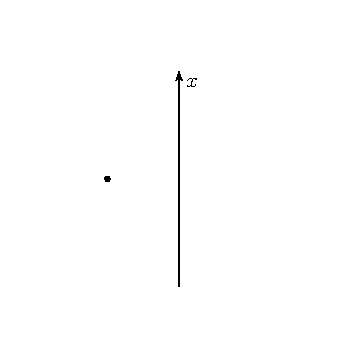
\includegraphics[scale=1.2]{chapter3-picture}
\par\end{centering}
\vspace{-1.4\baselineskip}
\caption{The disjoint domain represented by the type \lstinline!RootsOfQ!.\label{fig:RootsOfQ-disjoint-domain}}
\end{figure}

In the mathematical notation, a one-dimensional real space is denoted
by $\mathbb{R}$, a two-dimensional space by $\mathbb{R}^{2}$, and
a zero-dimensional space by $\mathbb{R}^{0}$. At first, we may think
that the mathematical representation of the type \lstinline!RootsOfQ!
is a union of the three sets, $\mathbb{R}^{0}\cup\mathbb{R}^{1}\cup\mathbb{R}^{2}$.
But an ordinary union of sets would not always work correctly because
we need to distinguish the parts of the union unambiguously, even
if some parts have the same type. For instance, the disjunctive type
shown in Example~\ref{subsec:disj-Example-rootsofq-2} cannot be
correctly represented by the mathematical union:
\[
\mathbb{R}^{0}\cup\mathbb{R}^{0}\cup\mathbb{R}^{1}\cup\mathbb{R}^{0}\cup\mathbb{R}^{1}\cup\mathbb{R}^{2}\quad,
\]
because $\mathbb{R}^{0}\cup\mathbb{R}^{0}=\mathbb{R}^{0}$ and $\mathbb{R}^{1}\cup\mathbb{R}^{1}=\mathbb{R}^{1}$,
so:
\[
\mathbb{R}^{0}\cup\mathbb{R}^{0}\cup\mathbb{R}^{1}\cup\mathbb{R}^{0}\cup\mathbb{R}^{1}\cup\mathbb{R}^{2}=\mathbb{R}^{0}\cup\mathbb{R}^{1}\cup\mathbb{R}^{2}\quad.
\]
For instance, this representation has no distinction between the cases
\lstinline!Linear(x)! and \lstinline!OneRootQ(x)!.

In Scala code, each part of a disjunctive type must be distinguished
by a unique name such as \lstinline!NoRoots!, \lstinline!OneRoot!,
and \lstinline!TwoRoots!. To represent this mathematically, we need
to attach a distinct label, or \textsf{``}tag\textsf{''}, to each part of the union.
Tags are symbols without any special meaning in mathematics. In Scala,
tags are names of case classes. Parts of the union are then represented
by sets of pairs such as $(\text{\texttt{OneRoot}},x)_{x\in\mathbb{R}^{1}}$.
Then the domain \lstinline!RootsOfQ! is expressed as:
\[
\text{\texttt{RootsOfQ}}=(\text{\texttt{NoRoots}},u)_{u\in\mathbb{R}^{0}}\cup(\text{\texttt{OneRoot}},x)_{x\in\mathbb{R}^{1}}\cup(\text{\texttt{TwoRoots}},\left(x,y\right))_{\left(x,y\right)\in\mathbb{R}^{2}}\quad.
\]
This is an ordinary union of mathematical sets, but each of the sets
has a unique tag, so no two values from different parts of the union
could possibly be equal. This kind of set is called a \index{tagged union!see \textsf{``}disjunctive type\textsf{''}}\textbf{tagged
union} (also a \textsf{``}disjoint union\textsf{''}\index{disjoint union!see \textsf{``}disjunctive type\textsf{''}}).
Each element of a tagged union is a pair of the form \lstinline!(tag, data)!,
where the tag uniquely identifies the part of the union, and the data
can have any chosen type such as $\mathbb{R}^{1}$. If we use tagged
unions, we cannot confuse different parts of the union even if their
data have the same type, because tags are required to be distinct.

Tagged unions are not often used in mathematics, but they are needed
in software engineering because real-life data is often described
by sets having several disjoint parts.

\paragraph{Named \texttt{Unit} types}

At first sight, it may seem strange that the zero-dimensional space
is represented by a set containing \emph{one} point. Why should we
not use an empty set (rather than a set with one element) to represent
the case where the equation has no real roots? The reason is that
we are required to represent not only the values of the roots but
also the information \emph{about} the existence of the roots. The
case with no real roots needs to be represented by some \emph{value}
of type \lstinline!RootsOfQ!. That value cannot be missing, which
would happen if we used an empty set to represent the no-roots case.
It is natural to use the named empty tuple \lstinline!NoRoots()!
to represent that case, just as we used a named $2$-tuple \lstinline!TwoRoots(x, y)!
to represent the case of two roots.

Consider the value $u$ used by the mathematical set $\left(\text{\texttt{NoRoots}},u\right)_{u\in\mathbb{R}^{0}}$.
Since $\mathbb{R}^{0}$ consists of a single point, there is only
\emph{one} possible value of $u$. Similarly, the \lstinline!Unit!
type in Scala has only one distinct value, written as \lstinline!()!.
A case class with no parts, such as \lstinline!NoRoots!, has only
one distinct value, written as \lstinline!NoRoots()!. The Scala value
\lstinline!NoRoots()! is fully analogous to the mathematical notation
$\left(\text{\texttt{NoRoots}},u\right)_{u\in\mathbb{R}^{0}}$.

So, case classes with no parts are similar to \lstinline!Unit! except
for an added name. For instance, \lstinline!NoRoots()! can be regarded
as the \lstinline!Unit! value \lstinline!()! with name \lstinline!NoRoots!.
For this reason, this book calls them \textsf{``}named unit\textsf{''} types.\index{unit type!named}

\subsection{Disjunctive types in other programming languages}

Disjunctive types and pattern matching turns out to be one of the
defining features of FP languages. Languages that were not designed
for functional programming do not support these features, while OCaml,
Haskell, F\#, Scala, Swift, and Rust support disjunctive types and
pattern matching as part of the language design. 

It is remarkable that named tuple types (also called \textsf{``}structs\textsf{''}
or \textsf{``}records\textsf{''}) are provided in almost every programming language,
while disjunctive types are almost never present except in languages
designed for the FP paradigm.\footnote{The programming languages Ada and Pascal support disjunctive types
but no other FP features.}

The \lstinline!union! types in C and C++ are not disjunctive types
because it is not possible to determine which part of the union is
represented by a given value. A \lstinline!union! declaration in
C looks like this:
\begin{lstlisting}[language=C]
union { int x; double y; long z; } i_d_l;
\end{lstlisting}
This type does not include any labels telling us which of the values
is present. Without a label, we (and the compiler) will not know whether
a given value of type \lstinline!i_d_l! represents an \lstinline!int!,
a \lstinline!double!, or a \lstinline!long!. This will lead to errors
that are hard to detect.

Programming languages of the C family (C, C++, Objective C, Java)
support \textbf{enumeration} (\lstinline!enum!) types\index{enumeration type},
which are a limited form of disjunctive types, and a \lstinline!switch!
operation, which is a limited form of pattern matching. An \lstinline!enum!
type declaration in Java looks like this:
\begin{lstlisting}[language=Java]
enum Color { RED, GREEN, BLUE; } 
\end{lstlisting}
In Scala, this is equivalent to a disjunctive type containing three
\emph{empty} tuples:
\begin{lstlisting}
sealed trait Color
final case class RED()   extends Color
final case class GREEN() extends Color
final case class BLUE()  extends Color
\end{lstlisting}
If we add extra data to the \lstinline!enum! types, allowing the
tuples to be non-empty, and extend the \lstinline!switch! expression
to be able to handle the extra data, we will recover the full functionality
of disjunctive types. A definition of \lstinline!RootsOfQ! could
then look like this: 
\begin{lstlisting}
enum RootsOfQ {                 // This is not valid in Java!
  NoRoots(), OneRoot(Double x), TwoRoots(Double x, Double y);
}
\end{lstlisting}
Scala 3 has a shorter a syntax for disjunctive types\footnote{\texttt{\href{https://dotty.epfl.ch/docs/reference/enums/adts.html}{https://dotty.epfl.ch/docs/reference/enums/adts.html}}}
that resembles Java\textsf{'}s \textsf{``}\lstinline!enum!\textsf{''}:
\begin{lstlisting}
enum RootsOfQ {
  case NoRoots
  case OneRoot(x: Double)
  case TwoRoots(x: Double, y: Double)
}
\end{lstlisting}
For comparison, the syntax for a disjunctive type equivalent to \lstinline!RootsOfQ!
in OCaml and Haskell is:
\begin{lstlisting}[language=Caml]
(* OCaml *)
type RootsOfQ = NoRoots | OneRoot of float | TwoRoots of float * float
\end{lstlisting}
\begin{lstlisting}[language=Haskell]
-- Haskell
data RootsOfQ = NoRoots | OneRoot Double | TwoRoots (Double, Double)
\end{lstlisting}
This is more concise than the Scala syntax. When reasoning about disjunctive
types, it is inconvenient to write out long type definitions. Chapter~\ref{chap:5-Curry-Howard}
will introduce a mathematical notation designed for efficient reasoning
about types. That notation is even more concise than the syntax of
Haskell or OCaml.

\subsection{Disjunctions and conjunctions in formal logic\label{subsec:Disjunctions-and-conjunctions}}

In logic, a \textbf{proposition\index{proposition (in logic)}} is
a logical formula that could be true or false. A \textbf{disjunction\index{disjunction (in logic)}}
of propositions $A$, $B$, $C$ is denoted by $A\vee B\vee C$ and
is true if and only if \emph{at least one} of $A$, $B$, $C$ is
true. A \textbf{conjunction}\index{conjunction (in logic)} of $A$,
$B$, $C$ is denoted by $A\wedge B\wedge C$ and is true if and only
if \emph{all} of the propositions $A$, $B$, $C$ are true.

There is a connection between disjunctive data types and logical disjunctions
of propositions. A value of the disjunctive data type \lstinline!RootsOfQ!
can be constructed only if we have one of the values \lstinline!NoRoots()!,
\lstinline!OneRoot(x)!, or \lstinline!TwoRoots(x, y)!. Let us now
rewrite the previous sentence as a logical formula. Denote by ${\cal CH}(A)$
the logical proposition \textsf{``}we ${\cal C}\!$an ${\cal H}\!$ave a value
of type \lstinline!A! here\textsf{''}, where by \textsf{``}here\textsf{''} we mean a particular
scope in a program. So, the proposition \textsf{``}the code \emph{can} compute
a value of type \lstinline!RootsOfQ!\textsf{''} is denoted by ${\cal CH}(\text{\texttt{RootsOfQ}})$.
We can then write the above sentence about \lstinline!RootsOfQ! as
a logical formula:
\begin{equation}
{\cal CH}(\text{\texttt{RootsOfQ}})={\cal CH}(\text{\texttt{NoRoots}})\vee{\cal CH}(\text{\texttt{OneRoot}})\vee{\cal CH}(\text{\texttt{TwoRoots}})\quad.\label{eq:curry-howard-example-disjunction}
\end{equation}

There is a similar connection between logical \emph{conjunctions}
and tuple types. Consider the named tuple (i.e., a case class) \lstinline!TwoRoots(x: Double, y: Double)!.
We can have a value of type \lstinline!TwoRoots! only if we have
two values of type \lstinline!Double!. Rewriting this sentence as
a logical formula, we get:
\[
{\cal CH}(\text{\texttt{TwoRoots}})={\cal CH}(\text{\texttt{Double}})\wedge{\cal CH}(\text{\texttt{Double}})\quad.
\]
Formal logic admits the simplification:
\[
{\cal CH}(\text{\texttt{Double}})\wedge{\cal CH}(\text{\texttt{Double}})={\cal CH}(\text{\texttt{Double}})\quad.
\]
However, no such simplification will be available in the general case,
e.g.:
\begin{lstlisting}
case class Data3(x: Int, y: String, z: Double)
\end{lstlisting}
For this type, we will have the formula:
\begin{equation}
{\cal CH}(\text{\texttt{Data3}})={\cal CH}(\text{\texttt{Int}})\wedge{\cal CH}(\text{\texttt{String}})\wedge{\cal CH}(\text{\texttt{Double}})\quad.\label{eq:curry-howard-example-case-class}
\end{equation}

We find that tuples are related to logical conjunctions in the same
way as disjunctive types are related to logical disjunctions. This
is the main reason for choosing the name \textsf{``}disjunctive types\textsf{''}.\footnote{Disjunctive types are also called sum types, co-product types, variants,
and tagged unions. This book uses the terms \textsf{``}disjunctive types\textsf{''}
and \textsf{``}co-product types\textsf{''} interchangeably.}

The correspondence between disjunctions, conjunctions, and data types
is explained in more detail in Chapter~\ref{chap:5-Curry-Howard}.
For now, we note that the operations of conjunction and disjunction
are not sufficient to produce all possible logical expressions. To
obtain a complete logic, it is also necessary to have the logical
implication $A\rightarrow B$ (\textsf{``}if $A$ is true than $B$ is true\textsf{''}).
It turns out that the implication $A\rightarrow B$ is related to
the function type \lstinline!A => B! in the same way as the disjunction
operation is related to disjunctive types and the conjunction to tuples.
In Chapter~\ref{chap:Higher-order-functions}, we will study function
types in depth.
